\chapter{Implementation and Results}
\label{ch:impl}

This chapter describes the software environment and implementation, how the system was tested, and the experimental results: overall performance under both protocols, statistical tests, per-ticker and FinMem-universe results, predictive content, ablations, sensitivity analyses, retrieval diagnostics, the LLM-backbone comparison, the extension models (GRU, Transformer, reinforcement learning, pattern analogues), portfolio construction, robustness and power analyses, and the evaluation of the application.

\section{Environment Setup}
\begin{itemize}
  \item \textbf{Hardware}: a laptop with an 8-core CPU and 8\,GB RAM; no GPU is required (FinBERT and MiniLM run on CPU; annotating 23{,}247 articles took about 50 minutes, a full replay of 16 memory configurations about 15 minutes).
  \item \textbf{Software}: Python 3.13, pandas, NumPy, SciPy, scikit-learn, LightGBM, PyTorch (CPU), Hugging Face Transformers and Sentence-Transformers, Matplotlib; the web server uses only the Python standard library and the front end is plain HTML, CSS and JavaScript with hand-written SVG charts.
  \item \textbf{External services}: Alpaca Market Data (news and SIP bars) and Alpaca paper trading, SEC EDGAR XBRL API, Groq and OpenRouter free tiers. Credentials are read from a local \texttt{.env} file that is excluded from version control.
  \item \textbf{Code organisation} (\texttt{src/agentic\_trade/study}): \texttt{data.py} (download, alignment, incremental refresh), \texttt{annotate.py}, \texttt{memory.py} (all memories and N1--N7 flags), \texttt{backtest.py} (day-major replay), \texttt{policies.py}, \texttt{evaluation.py}, \texttt{pipeline.py} (protocols), \texttt{llm\_agent.py}, \texttt{figures.py}; the extension experiments are in \texttt{study/extensions.py}. The application consists of \texttt{dashboard\_server.py} (HTTP API), \texttt{agent\_service.py} (research agent), \texttt{autopilot.py} (budget, guardrails, permission modes, scheduler), \texttt{analytics.py} (pattern analogues, risk, correlation, allocation, Monte Carlo), \texttt{algorithms.py} (algorithm board and Q-learning agent) and \texttt{credentials.py} (API-key management), and a front end split into \texttt{core.js} (navigation, global stock, language, theme), \texttt{i18n.js} (about 750 English/Bangla strings), \texttt{charts.js}, \texttt{trade.js}, \texttt{autopilot.js}, \texttt{analytics.js}, \texttt{app.js} and \texttt{credentials.js}. Scripts \texttt{build\_dataset.py}, \texttt{run\_study.py}, \texttt{run\_llm\_study.py}, \texttt{run\_extensions.py}, \texttt{make\_extension\_figures.py}, \texttt{export\_latex\_tables.py}, \texttt{export\_extension\_tables.py} and \texttt{capture\_app\_screens.py} reproduce the dataset, results, figures, tables and screenshots in this report.
\end{itemize}

The replay is \emph{day-major}: all tickers advance together, so information shared across tickers (source credibility) can only contain outcomes that were already public. Each memory keeps its items in pre-allocated NumPy arrays, so a retrieval is a masked matrix--vector product followed by a per-layer partial sort.

\section{Testing and Evaluation}
The repository contains \testcount{} automated tests (pytest), all passing. The study-specific tests check:
\begin{itemize}
  \item point-in-time alignment (an article at 15:59 New York time belongs to the same session, at 16:01 to the next; weekend news to Monday);
  \item that retrieval never returns future items and that FinMem retrieves per layer;
  \item FinMem's decay constants, purge rule and access-counter promotion with recency reset;
  \item that duplicates are merged and contradictions retired only in our memory, never in FinMem;
  \item credibility shrinkage (an unseen author inherits the category estimate);
  \item episodic recall requiring at least five similar episodes;
  \item Hold-keeps-position semantics and transaction-cost accounting;
  \item non-overlapping splits, metric and Holm-correction helpers;
  \item the application's consensus rule (agreement, disagreement, abstention, weak price signals) and that the agent brief is built from the research memory.
\end{itemize}
Tests added for the extensions and the application check:
\begin{itemize}
  \item the Q-learning agent cannot look ahead: changing the last five days of prices leaves every earlier decision and the learning curve unchanged, and it is deterministic for a fixed seed;
  \item pattern analogues only use windows whose outcome was already known and never overlap the window being matched; an always-long analogue strategy reproduces buy-and-hold exactly;
  \item the guardrail sizes buys by the tightest of target, cash above reserve and order cap; blocks buys (but not exits) after the daily-loss or drawdown limit; enforces allowed stocks and trades per day; and the emergency stop cancels the queue and prevents re-enabling;
  \item every permission mode routes decisions as specified, approvals are re-checked and proposals expire;
  \item budget-split plans respect the reserve and the per-stock cap for every method, and their rebalancing amounts are consistent with current holdings;
  \item API keys are validated before saving, stored with owner-only permissions, never returned unmasked, and the endpoints refuse cross-origin and foreign-host requests;
  \item the experience log of the algorithm board is internally consistent (a long position is ``right'' exactly when the next-day return is positive).
\end{itemize}
Legacy tests cover the paper-trading adapter, risk limits, LLM output parsing and the dashboard APIs. Every view of the application was also exercised end to end in a headless browser in both languages and both themes, on desktop and phone widths, with the browser console checked for errors. The front-end dictionary is checked automatically: every key used in the HTML or JavaScript exists in both languages and every placeholder appears in both translations.

\section{Results and Discussion}

\subsection{Overall performance}
Table~\ref{tab:main} reports the primary rolling protocol and Figure~\ref{fig:equity} the equity curves. Among the three memory architectures, ours has the highest Sharpe ratio, the smallest loss and the smallest drawdown; FinMem and flat retrieval behave almost identically. However, all three news-memory policies lose money over the period, while buy-and-hold and, above all, the price-only LightGBM earn positive returns. Adding memory features to LightGBM \emph{reduces} its Sharpe ratio, indicating that the memory features mostly add noise for a tree model fitted on a few thousand observations.

\begin{table}[ht]
\centering
\caption{Ten-stock equal-weight portfolio, rolling walk-forward protocol (2025-12-01 to 2026-10-26, 227 sessions), net of 5\,bps. Best value per column in bold.}
\label{tab:main}
\small
\begin{tabular}{lrrrrrrr}
\hline
Strategy & CR (\%) & Sharpe & Sortino & Ann. Vol (\%) & MDD (\%) & Win (\%) & Turnover \\
\hline
Buy \& Hold & 11.15 & 0.61 & 0.96 & 23.82 & -16.50 & 50.2 & 0.00 \\
Momentum (1d) & -10.12 & -0.59 & -0.92 & 17.58 & -18.98 & 51.5 & 0.56 \\
TS-Momentum (20d) & -16.17 & -0.91 & -1.25 & 19.44 & -26.85 & 50.2 & 0.15 \\
Mean-Reversion (5d) & -4.54 & -0.21 & -0.30 & 17.22 & -21.57 & 48.0 & 0.30 \\
MA-Crossover & -3.37 & -0.12 & -0.16 & 18.02 & -19.62 & 53.3 & 0.17 \\
Daily News Sentiment & -22.24 & -2.26 & -3.11 & 12.05 & -23.32 & 42.7 & 0.38 \\ \hline
LogReg (price) & -21.54 & -1.39 & -2.13 & 18.20 & -29.66 & 47.1 & 0.20 \\
LGBM (price) & \textbf{19.40} & \textbf{1.15} & \textbf{1.91} & 18.59 & -17.15 & 54.2 & 0.70 \\
LGBM (price+FinMem) & 5.63 & 0.42 & 0.68 & 18.27 & -13.05 & 52.4 & 0.66 \\
LGBM (price+Ours) & 6.16 & 0.44 & 0.71 & 19.01 & \textbf{-11.03} & 51.1 & 0.60 \\ \hline
Plain RAG & -9.45 & -0.65 & -0.97 & 15.13 & -21.14 & 49.3 & 0.16 \\
FinMem & -10.98 & -0.72 & -1.03 & 16.11 & -19.69 & 48.5 & 0.07 \\
Ours & -3.56 & -0.20 & -0.30 & 14.84 & -15.18 & 49.3 & 0.06 \\
\hline
\end{tabular}
\end{table}


\begin{figure}[H]
\centering
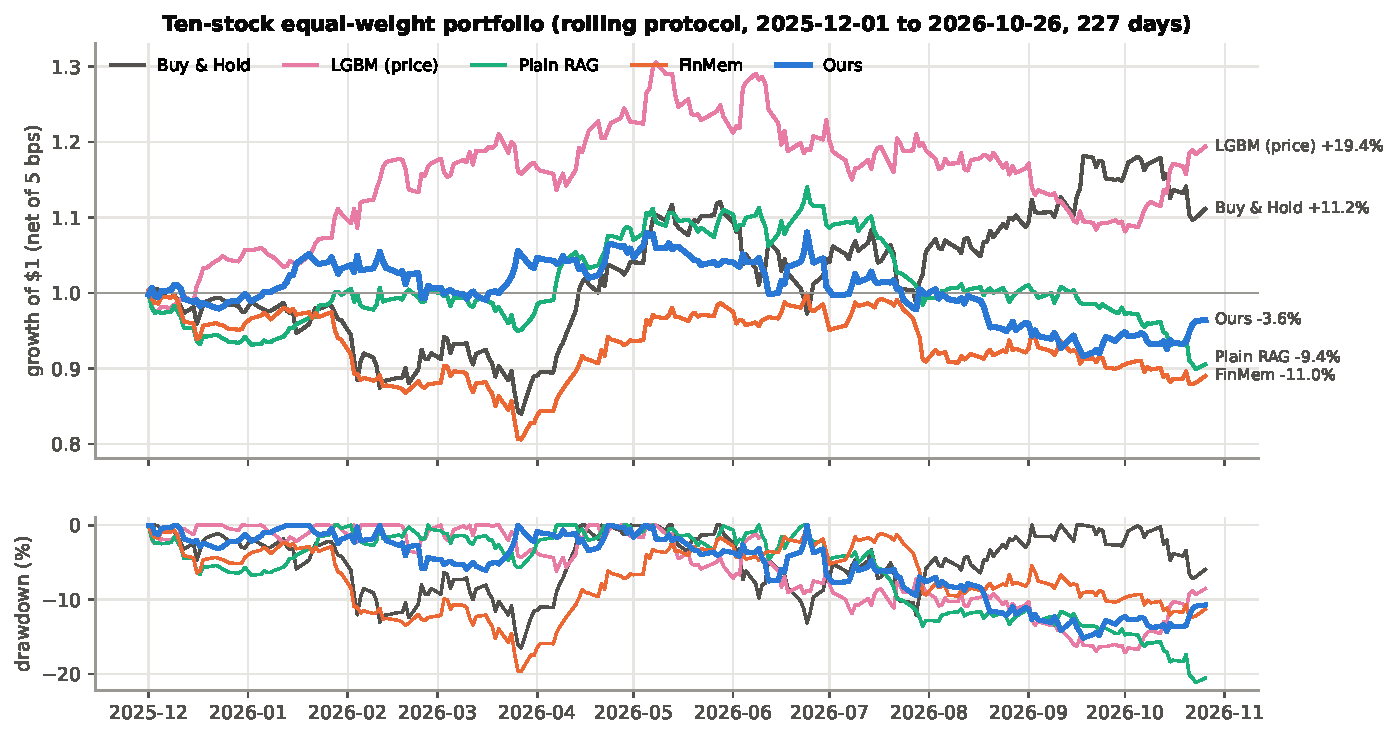
\includegraphics[width=\textwidth]{fig03_equity_portfolio.pdf}
\caption{Equal-weight ten-stock portfolio under the rolling protocol, net of costs, with drawdowns.}
\label{fig:equity}
\end{figure}

Two properties explain much of the gap to buy-and-hold. First, our memory abstains (keeps its position instead of acting on the signal) on 49\% of ticker-days because the episodic memory reports that similar situations were mis-signalled. Second, because Hold keeps the previous position, the memory policies are always invested, and ours is short on 58\% of ticker-days (FinMem 29\%, Plain RAG 43\%) in a market that rose over the period: its portfolio beta is $-0.33$ against $+0.64$ for FinMem (Figure~\ref{fig:positions}).

\begin{figure}[H]
\centering
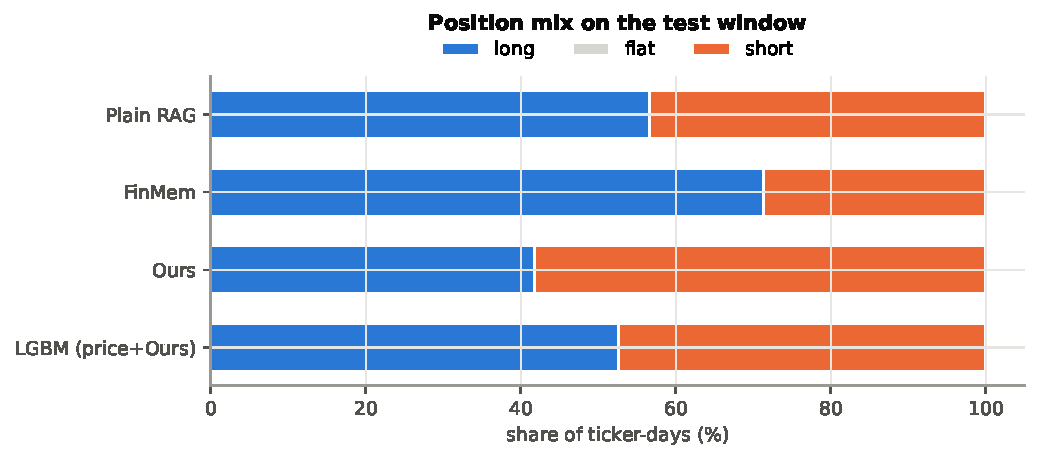
\includegraphics[width=0.75\textwidth]{fig17_positions.pdf}
\caption{Share of long, flat and short ticker-days in the test period.}
\label{fig:positions}
\end{figure}

\subsection{Statistical significance}
Table~\ref{tab:tests} compares ours with every baseline. Ours earns 3.4 basis points per day more than FinMem and has a Sharpe ratio higher by about 0.5, but the 95\% bootstrap interval of the difference contains zero and the Wilcoxon test is far from significance ($p=0.39$). The only Holm-significant differences are against the 1-day momentum rule and against trading on the day's headline tone without memory, i.e.\ memory is significantly better than reacting to today's news alone. Figure~\ref{fig:bootstrap} shows the bootstrap distributions.

\begin{table}[ht]
\centering
\caption{Ours versus every baseline on pooled (ticker, date) daily returns, rolling protocol. $\Delta$ = Ours $-$ baseline; CI from a 10-day moving-block bootstrap (5{,}000 resamples); Holm-adjusted Wilcoxon $p$; DM = Diebold--Mariano.}
\label{tab:tests}
\small
\begin{tabular}{lrrcrrr}
\hline
Baseline & $\Delta$ bps/day & $\Delta$Sharpe & 95\% CI & Wilcoxon $p$ & Holm $p$ & DM $p$ \\
\hline
Momentum (1d) & +2.9 & +0.39 & [-2.44, 2.85] & 0.000 & 0.000 & 0.723 \\
Daily News Sentiment & +9.6 & +2.06 & [-0.51, 4.38] & 0.000 & 0.001 & 0.164 \\
LGBM (price+FinMem) & -4.2 & -0.62 & [-3.34, 1.79] & 0.015 & 0.154 & 0.626 \\
LGBM (price) & -9.7 & -1.35 & [-3.99, 1.05] & 0.061 & 0.545 & 0.272 \\
LGBM (price+Ours) & -4.5 & -0.64 & [-2.92, 1.27] & 0.070 & 0.561 & 0.585 \\
LogReg (price) & +8.9 & +1.19 & [-1.18, 3.88] & 0.112 & 0.787 & 0.300 \\
TS-Momentum (20d) & +5.9 & +0.71 & [-1.68, 2.92] & 0.160 & 0.963 & 0.430 \\
Mean-Reversion (5d) & +0.3 & +0.02 & [-3.19, 2.67] & 0.308 & 1.000 & 0.973 \\
FinMem & +3.4 & +0.52 & [-2.73, 3.12] & 0.388 & 1.000 & 0.643 \\
MA-Crossover & -0.3 & -0.08 & [-2.16, 1.79] & 0.421 & 1.000 & 0.968 \\
Plain RAG & +2.8 & +0.46 & [-2.35, 2.36] & 0.426 & 1.000 & 0.683 \\
Buy \& Hold & -6.9 & -0.81 & [-4.11, 1.76] & 0.774 & 1.000 & 0.452 \\
\hline
\end{tabular}
\end{table}


\begin{figure}[H]
\centering
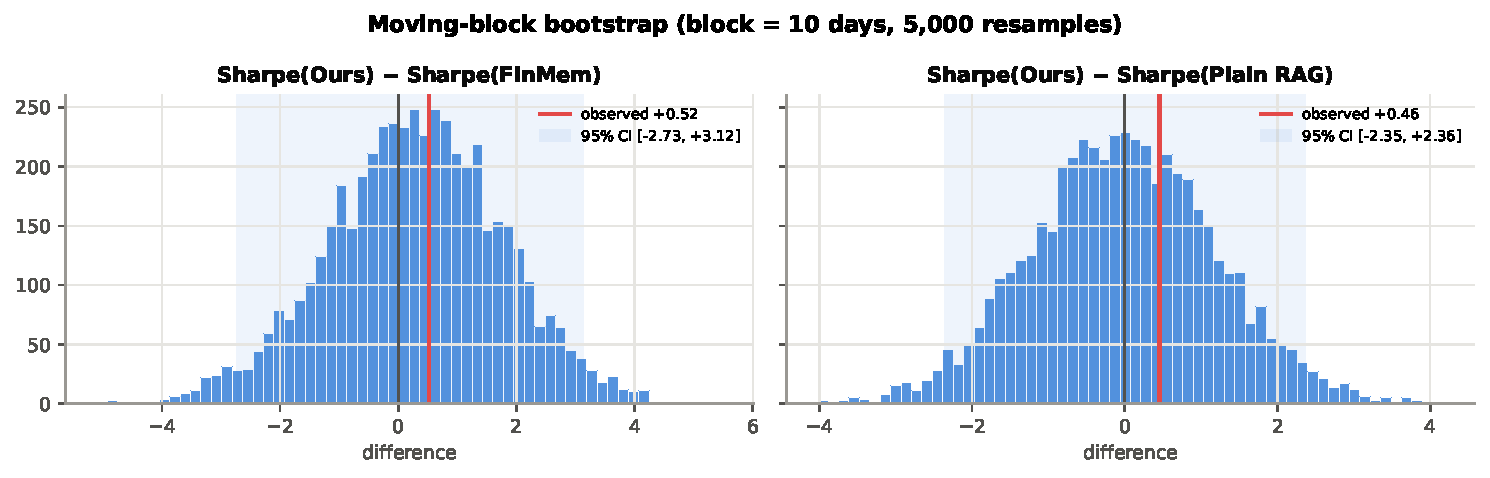
\includegraphics[width=\textwidth]{fig15_bootstrap.pdf}
\caption{Moving-block bootstrap distribution of the Sharpe difference between ours and FinMem (left) and Plain RAG (right).}
\label{fig:bootstrap}
\end{figure}

\subsection{FinMem's own stocks and per-ticker results}
On the five stocks FinMem was designed and evaluated on (Table~\ref{tab:finmem5}, Figure~\ref{fig:finmem5}), the difference is larger: FinMem and Plain RAG lose about 29\% while ours gains 3.5\%, also beating buy-and-hold ($-11.6\%$). Per ticker (Table~\ref{tab:perticker}, Figure~\ref{fig:heatmap}) the picture is mixed: ours is the best memory on NFLX, MSFT and COIN, but worse than FinMem on AMD, META, NVDA and TSLA. Such dispersion is expected when the underlying signal is weak.

\begin{table}[ht]
\centering
\caption{Equal-weight portfolio of FinMem's five stocks (TSLA, NFLX, AMZN, MSFT, COIN), rolling protocol, net of 5\,bps.}
\label{tab:finmem5}
\begin{tabular}{lrrrr}
\hline
System & CR (\%) & Sharpe & MDD (\%) & Ann. Vol (\%) \\
\hline
Buy \& Hold & -11.58 & -0.34 & -24.10 & 28.23 \\
Plain RAG & -28.82 & -1.59 & -31.61 & 22.20 \\
FinMem & -28.62 & -1.59 & -29.01 & 22.03 \\
Ours & \textbf{3.52} & \textbf{0.28} & \textbf{-20.03} & 22.35 \\
\hline
\end{tabular}
\end{table}


\begin{figure}[H]
\centering
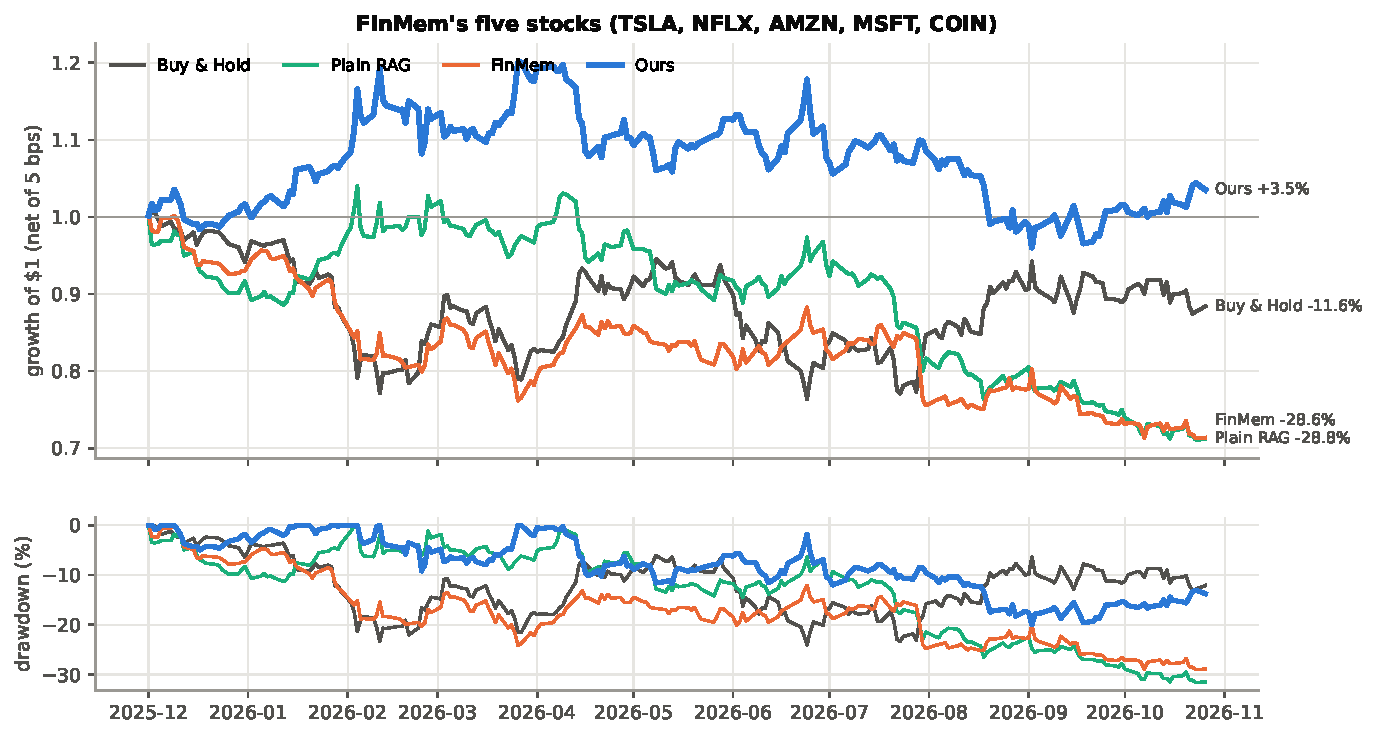
\includegraphics[width=\textwidth]{fig04_equity_finmem5.pdf}
\caption{Portfolio of FinMem's five stocks under the rolling protocol.}
\label{fig:finmem5}
\end{figure}

\begin{table}[ht]
\centering
\caption{Per-ticker Sharpe ratio, rolling protocol (net of costs).}
\label{tab:perticker}
\small
\setlength{\tabcolsep}{4pt}
\begin{tabular}{lrrrrrrrrrr}
\hline
Strategy & AAPL & AMD & AMZN & COIN & GOOGL & META & MSFT & NFLX & NVDA & TSLA \\
\hline
Buy \& Hold & 1.05 & 1.86 & 0.42 & -0.38 & 0.23 & 0.13 & 0.47 & -1.52 & 0.77 & 0.09 \\
LGBM (price) & -0.92 & 0.63 & 0.69 & 0.68 & 0.57 & 0.18 & -1.22 & -0.06 & 2.13 & 1.38 \\
Plain RAG & 0.75 & 0.26 & -0.76 & -1.55 & 1.86 & -0.40 & 0.31 & 0.94 & 0.03 & -1.90 \\
FinMem & 0.56 & 0.86 & -0.54 & -1.73 & -1.61 & 0.09 & 0.05 & 0.26 & 0.84 & -0.99 \\
Ours & 0.66 & 0.12 & -0.52 & 0.08 & 0.27 & -1.66 & 0.64 & 2.33 & -0.64 & -1.39 \\
\hline
\end{tabular}
\end{table}


\begin{figure}[H]
\centering
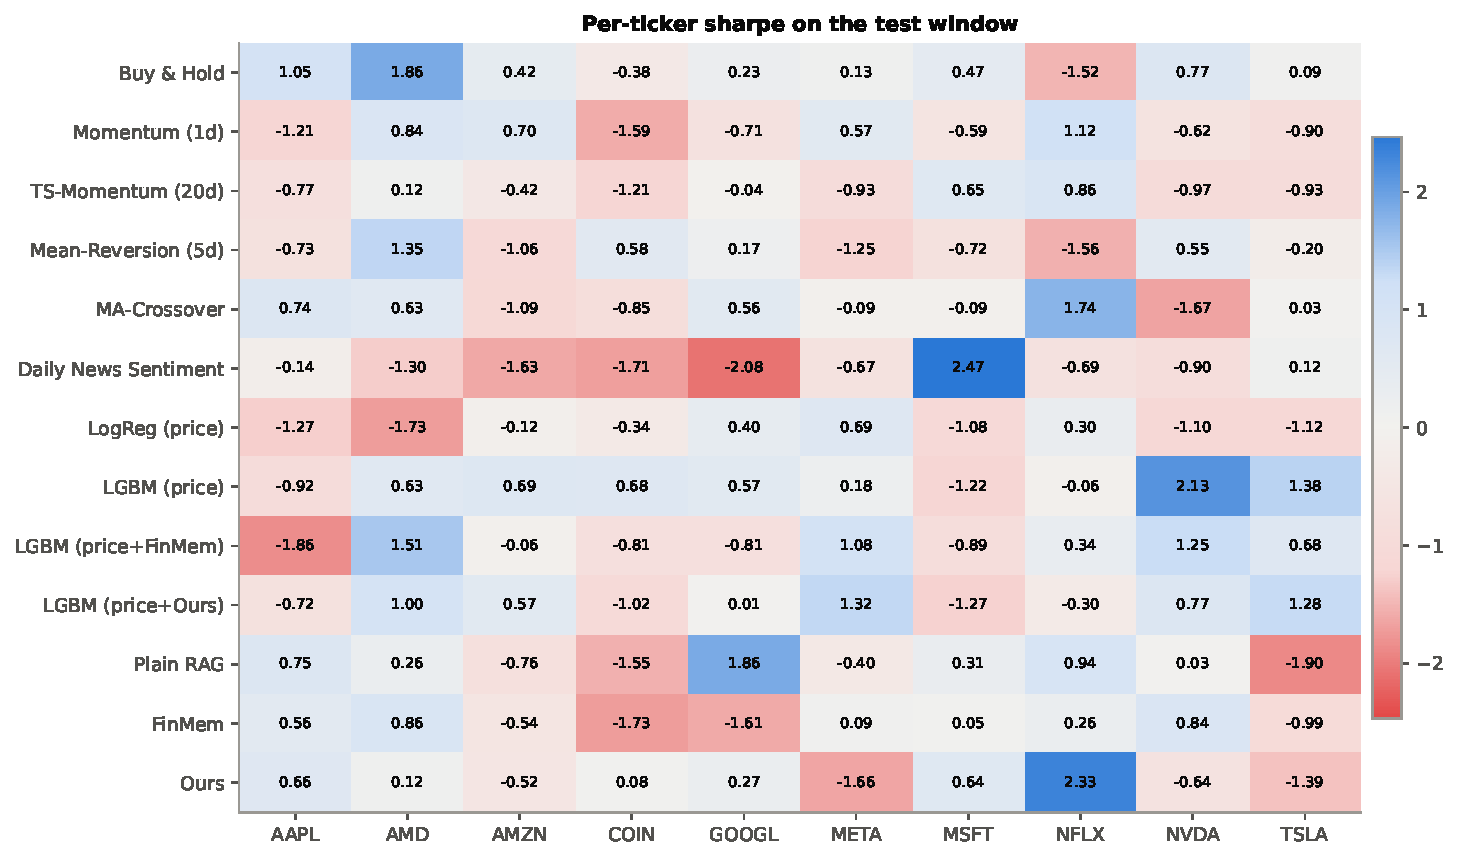
\includegraphics[width=\textwidth]{fig06_heatmap_sharpe.pdf}
\caption{Per-ticker Sharpe ratio of all strategies.}
\label{fig:heatmap}
\end{figure}

\begin{figure}[H]
\centering
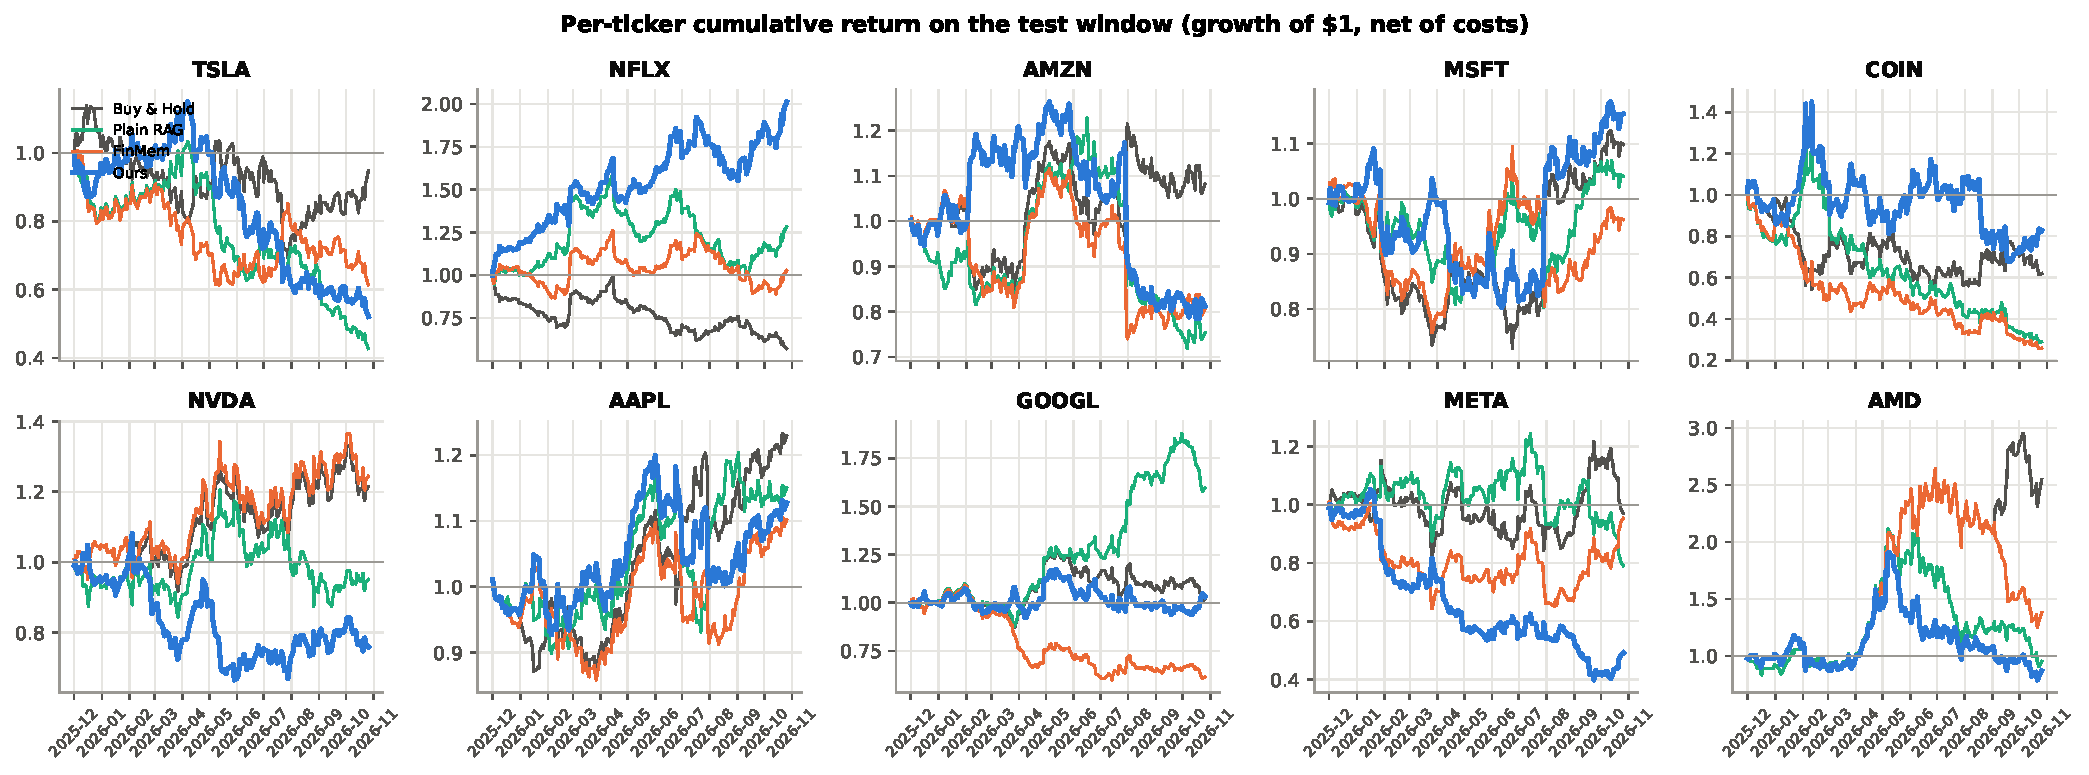
\includegraphics[width=\textwidth]{fig05_per_ticker.pdf}
\caption{Per-ticker cumulative returns of buy-and-hold and the three memories.}
\label{fig:perticker}
\end{figure}

\subsection{Predictive content of the memory}
Table~\ref{tab:icops} shows the Spearman IC between each memory signal and the next-day market-adjusted return. All values are within $\pm 0.04$ and none is significant at 5\%; flat retrieval of the most recent headlines is, if anything, slightly contrarian ($-0.037$, $p=0.08$), consistent with short-term reversal after news~\cite{chan2003stock,jegadeesh1990evidence}. This is the central empirical finding of the re-evaluation: in 2025--26, for these liquid large caps, the polarity of the retrieved news carries almost no information about the next day's move once it is public at the close, and FinMem's premise that better-organised news memory yields better daily trades does not hold on this data. The rolling 40-day Sharpe ratio (Figure~\ref{fig:rolling}) and monthly returns (Figure~\ref{fig:monthly}) confirm that relative performance changes sign across regimes.

\begin{table}[ht]
\centering
\caption{Predictive content of each memory signal (Spearman IC vs.\ next-day market-adjusted return, rolling test period) and memory operations over the full run (ten tickers).}
\label{tab:icops}
\small
\begin{tabular}{lrrrrrrrr}
\hline
System & IC & $p$ & IC (cross-sect.) & Items & Merged & Retired & Promoted & Purged \\
\hline
Plain RAG & -0.037 & 0.08 & -0.040 & 36,177 & 0 & 0 & 0 & 0 \\
FinMem & -0.000 & 0.99 & -0.007 & 36,177 & 0 & 0 & 1,221 & 32,625 \\
Ours & +0.003 & 0.90 & +0.015 & 33,917 & 2,260 & 667 & 1,510 & 29,417 \\
\hline
\end{tabular}
\end{table}


\begin{figure}[H]
\centering
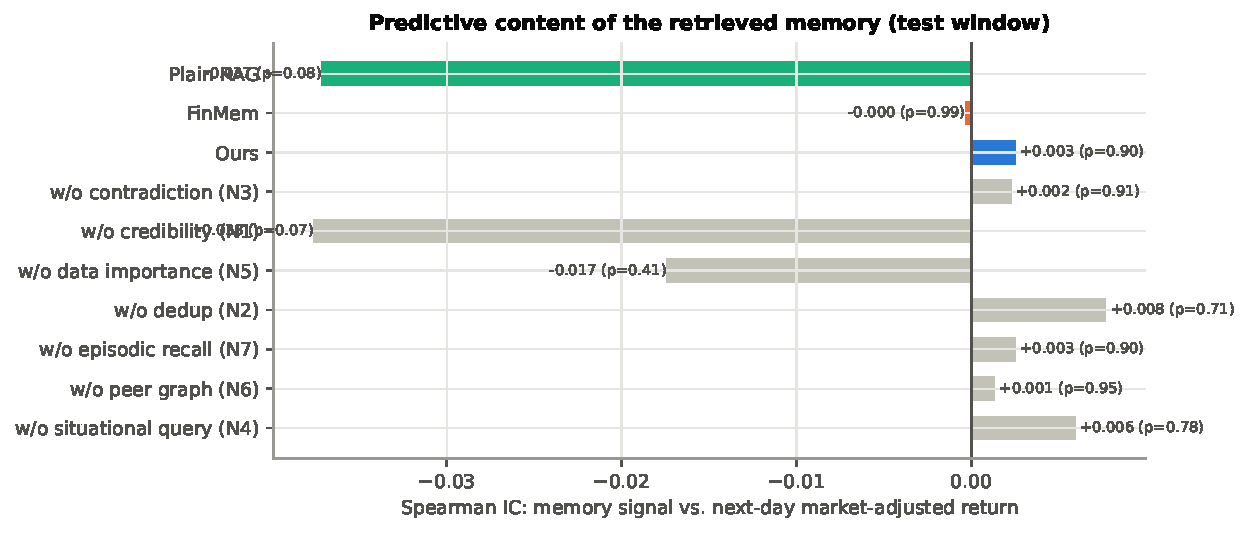
\includegraphics[width=0.85\textwidth]{fig12_information_coefficient.pdf}
\caption{Information coefficient of the memory signals, including ablated variants.}
\label{fig:ic}
\end{figure}

\begin{figure}[H]
\centering
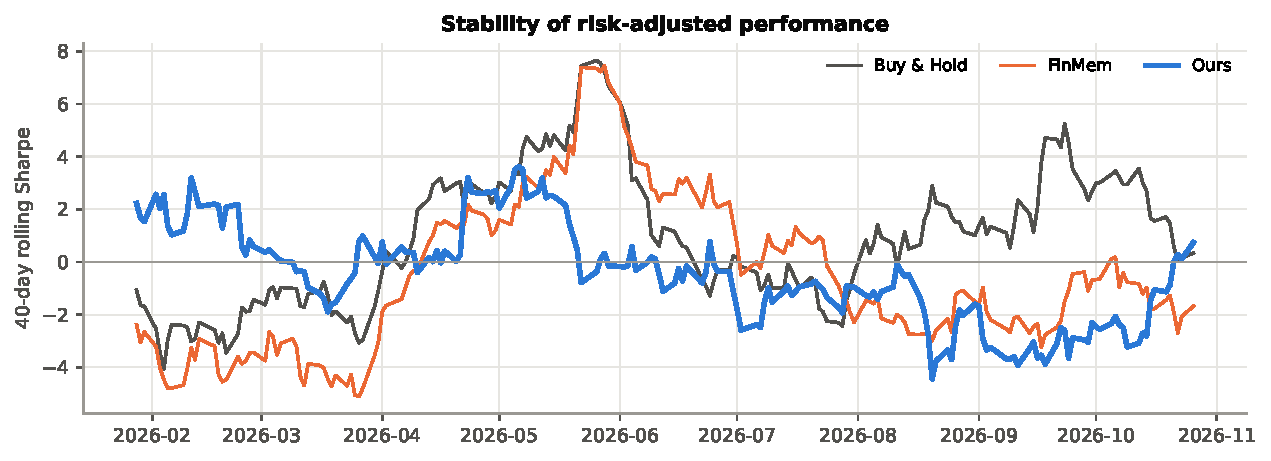
\includegraphics[width=\textwidth]{fig11_rolling_sharpe.pdf}
\caption{40-day rolling Sharpe ratio.}
\label{fig:rolling}
\end{figure}

\begin{figure}[H]
\centering
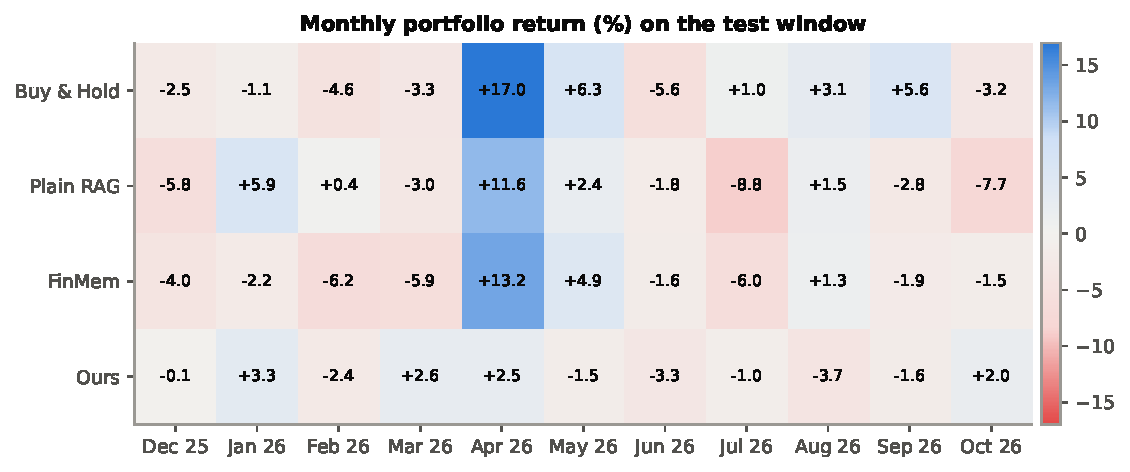
\includegraphics[width=0.85\textwidth]{fig16_monthly.pdf}
\caption{Monthly portfolio returns.}
\label{fig:monthly}
\end{figure}

\subsection{Ablation study}
Table~\ref{tab:ablation} and Figure~\ref{fig:ablation} remove one component at a time. The situational query (N4), the peer graph (N6) and data-driven importance (N5) contribute most to the Sharpe ratio. Removing episodic recall (N7) slightly increases the Sharpe ratio but raises the maximum drawdown from $-15.2\%$ to $-25.1\%$, and removing credibility (N1) raises it to $-18.6\%$: these two components act mainly as risk controls. Removing duplicate consolidation (N2) or contradiction retirement (N3) \emph{improves} the threshold policy; their benefit is in the quality and diversity of the context rather than in the aggregated polarity, which matters for an LLM reader but not for a polarity average. Given the noise level, differences of a few tenths of a Sharpe point should not be over-interpreted.

\begin{table}[ht]
\centering
\caption{Component ablation of our memory (rolling protocol). Each row removes one component; ``FinMem'' removes all of them.}
\label{tab:ablation}
\begin{tabular}{lrrrrr}
\hline
Variant & CR (\%) & Sharpe & $\Delta$Sharpe & MDD (\%) & IC \\
\hline
Ours & -3.56 & -0.20 &  & -15.18 & +0.003 \\
w/o contradiction (N3) & 0.78 & 0.13 & +0.33 & -12.79 & +0.002 \\
w/o credibility (N1) & -3.90 & -0.22 & -0.03 & -18.62 & -0.038 \\
w/o data importance (N5) & -6.60 & -0.47 & -0.28 & -13.96 & -0.017 \\
w/o dedup (N2) & -0.75 & 0.02 & +0.22 & -15.91 & +0.008 \\
w/o episodic recall (N7) & -2.47 & -0.10 & +0.10 & -25.10 & +0.003 \\
w/o peer graph (N6) & -7.75 & -0.52 & -0.32 & -19.29 & +0.001 \\
w/o situational query (N4) & -11.91 & -0.90 & -0.70 & -20.43 & +0.006 \\
FinMem & -10.98 & -0.72 & -0.52 & -19.69 & -0.000 \\
\hline
\end{tabular}
\end{table}


\begin{figure}[H]
\centering
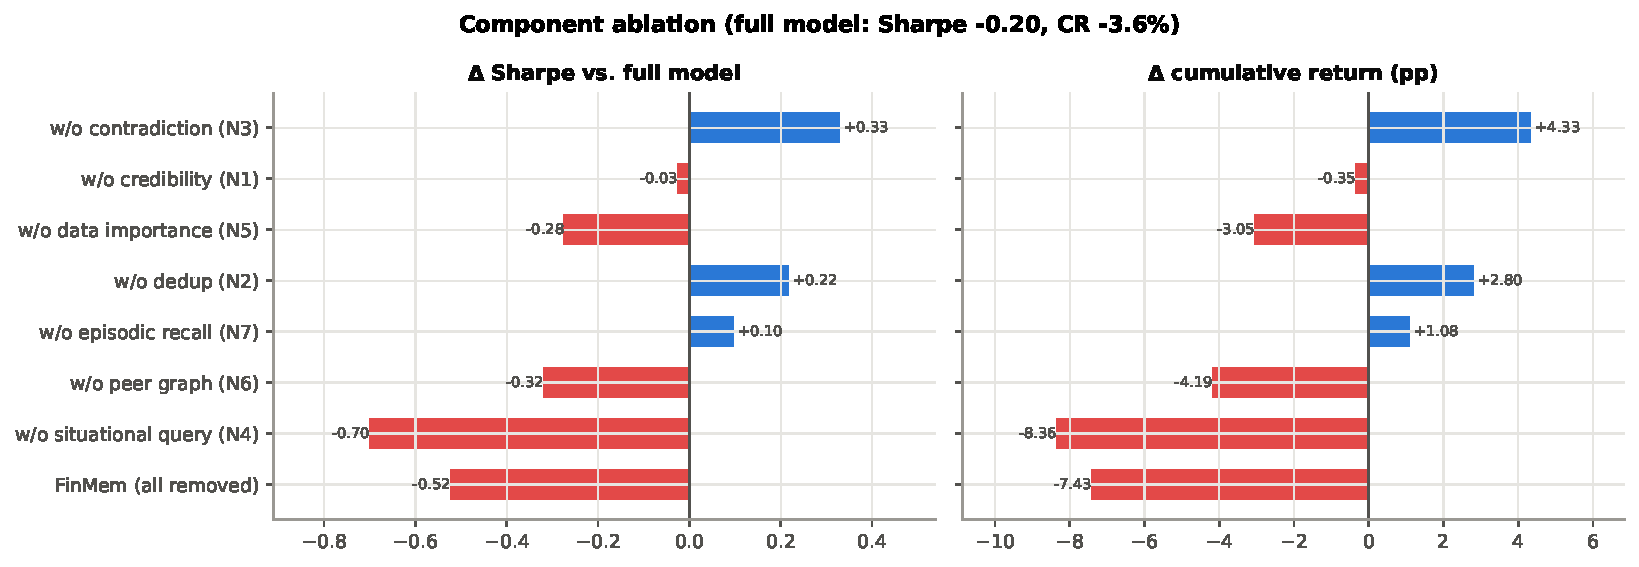
\includegraphics[width=\textwidth]{fig08_ablation.pdf}
\caption{Change in Sharpe ratio and cumulative return when a component is removed.}
\label{fig:ablation}
\end{figure}

\subsection{Sensitivity analyses}
\paragraph{Working-memory capacity.} Table~\ref{tab:topk} and Figure~\ref{fig:topk} vary $K$. Performance is non-monotonic and the spread across $K$ (FinMem: $-0.72$ to $2.27$) is larger than the difference between architectures at $K=5$; with $K=1$ FinMem performs best of all configurations. We kept FinMem's $K=5$ fixed in advance and report this sensitivity as a warning: choosing $K$ on the test period would be a form of selection bias~\cite{bailey2014deflated}.

\begin{table}[ht]
\centering
\caption{Sensitivity to working-memory capacity (top-$K$ per layer), Sharpe ratio, rolling protocol.}
\label{tab:topk}
\begin{tabular}{lrrrr}
\hline
System & $K=1$ & $K=3$ & $K=5$ & $K=10$ \\
\hline
FinMem & 2.27 & 0.11 & -0.72 & -0.38 \\
Ours & 0.51 & -0.64 & -0.20 & -0.46 \\
\hline
\end{tabular}
\end{table}


\begin{figure}[H]
\centering
\begin{minipage}{0.48\textwidth}\centering
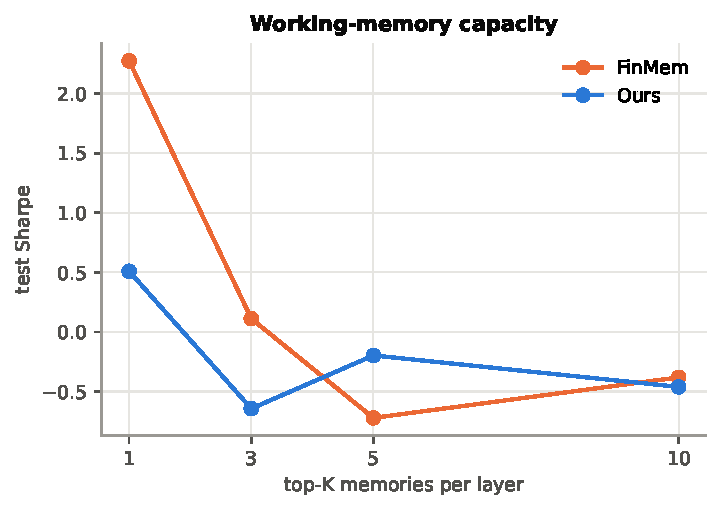
\includegraphics[width=\textwidth]{fig09_topk.pdf}
\caption{Sharpe ratio versus top-$K$.}
\label{fig:topk}
\end{minipage}\hfill
\begin{minipage}{0.48\textwidth}\centering
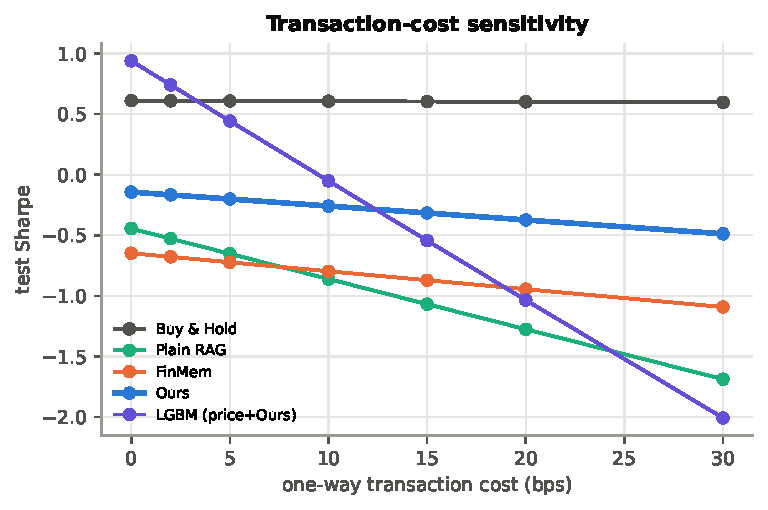
\includegraphics[width=\textwidth]{fig10_costs.pdf}
\caption{Sharpe ratio versus transaction cost.}
\label{fig:costs}
\end{minipage}
\end{figure}

\paragraph{Transaction costs.} The memory policies trade rarely (turnover 0.06--0.16 position units per day). Ours remains the best memory at every cost level from 0 to 30\,bps, while FinMem overtakes Plain RAG above about 8\,bps because Plain RAG trades twice as often (Figure~\ref{fig:costs}). The high-turnover LightGBM with memory features falls from a Sharpe ratio of 0.94 without costs to $-2.0$ at 30\,bps.

\paragraph{Fixed-split protocol.} Under the single test window of FinMem's design (Table~\ref{tab:fixed}), the ranking reverses: FinMem's validation-selected threshold ($\theta=0.4$) makes it almost always long, which matches buy-and-hold in a rising market, while ours, with $\theta=0.15$, trades more and loses. On the validation period itself ours had the highest IC of the three memories (0.087 versus 0.065 for FinMem and $-0.006$ for Plain RAG), and this ranking did not survive into the test period. The contrast between the two protocols is the strongest argument for walk-forward evaluation of trading agents.

\begin{table}[ht]
\centering
\caption{Ten-stock portfolio, fixed-split protocol (test 2026-05-01 to 2026-10-26, 123 sessions).}
\label{tab:fixed}
\small
\begin{tabular}{lrrrrrrr}
\hline
Strategy & CR (\%) & Sharpe & Sortino & Ann. Vol (\%) & MDD (\%) & Win (\%) & Turnover \\
\hline
Buy \& Hold & 6.79 & 0.68 & 1.07 & 23.89 & -13.19 & 51.2 & 0.01 \\
Momentum (1d) & -16.22 & -2.06 & -3.21 & 16.89 & -18.35 & 46.3 & 0.56 \\
TS-Momentum (20d) & -13.64 & -1.38 & -2.02 & 20.30 & -26.85 & 49.6 & 0.16 \\
Mean-Reversion (5d) & \textbf{14.97} & \textbf{1.80} & 2.47 & 16.67 & \textbf{-5.29} & 53.7 & 0.30 \\
MA-Crossover & -7.86 & -0.83 & -1.15 & 18.23 & -19.62 & 49.6 & 0.17 \\
Daily News Sentiment & -8.76 & -1.41 & -2.12 & 12.76 & -12.67 & 42.3 & 0.35 \\ \hline
LogReg (price) & -4.47 & -0.35 & -0.56 & 20.86 & -11.90 & 49.6 & 0.05 \\
LGBM (price) & -8.55 & -0.95 & -1.70 & 17.61 & -21.03 & 48.0 & 0.60 \\
LGBM (price+FinMem) & 11.95 & 1.46 & \textbf{2.68} & 16.76 & -6.03 & 48.8 & 0.59 \\
LGBM (price+Ours) & -8.18 & -0.94 & -1.48 & 16.98 & -16.66 & 51.2 & 0.64 \\ \hline
Plain RAG & -10.64 & -1.34 & -2.02 & 16.25 & -18.05 & 46.3 & 0.11 \\
FinMem & 5.25 & 0.67 & 1.10 & 18.08 & -10.60 & 52.0 & 0.01 \\
Ours & -15.37 & -2.21 & -3.13 & 14.97 & -17.95 & 44.7 & 0.07 \\
\hline
\end{tabular}
\end{table}


\subsection{Retrieval diagnostics}
Figure~\ref{fig:retrieval} characterises the retrieved context. Flat retrieval returns the most redundant context (mean pairwise similarity 0.45, against 0.36 for FinMem and 0.37 for ours) and only same-day news; FinMem's context is the oldest (mean age 58 days, dominated by filings and promoted items); ours retrieves fresher memories (26 days) while still covering all three layers. Over the run our memory merged 2{,}260 re-reported stories and retired 667 contradicted ones (Table~\ref{tab:icops}, Figure~\ref{fig:memdyn}). Learned credibility (Figure~\ref{fig:cred}) stays close to 0.5 for most categories; analyst notes (0.45) are the least reliable next-day guide and options-activity reports the most (0.64, but with only 80 observations).

\begin{figure}[H]
\centering
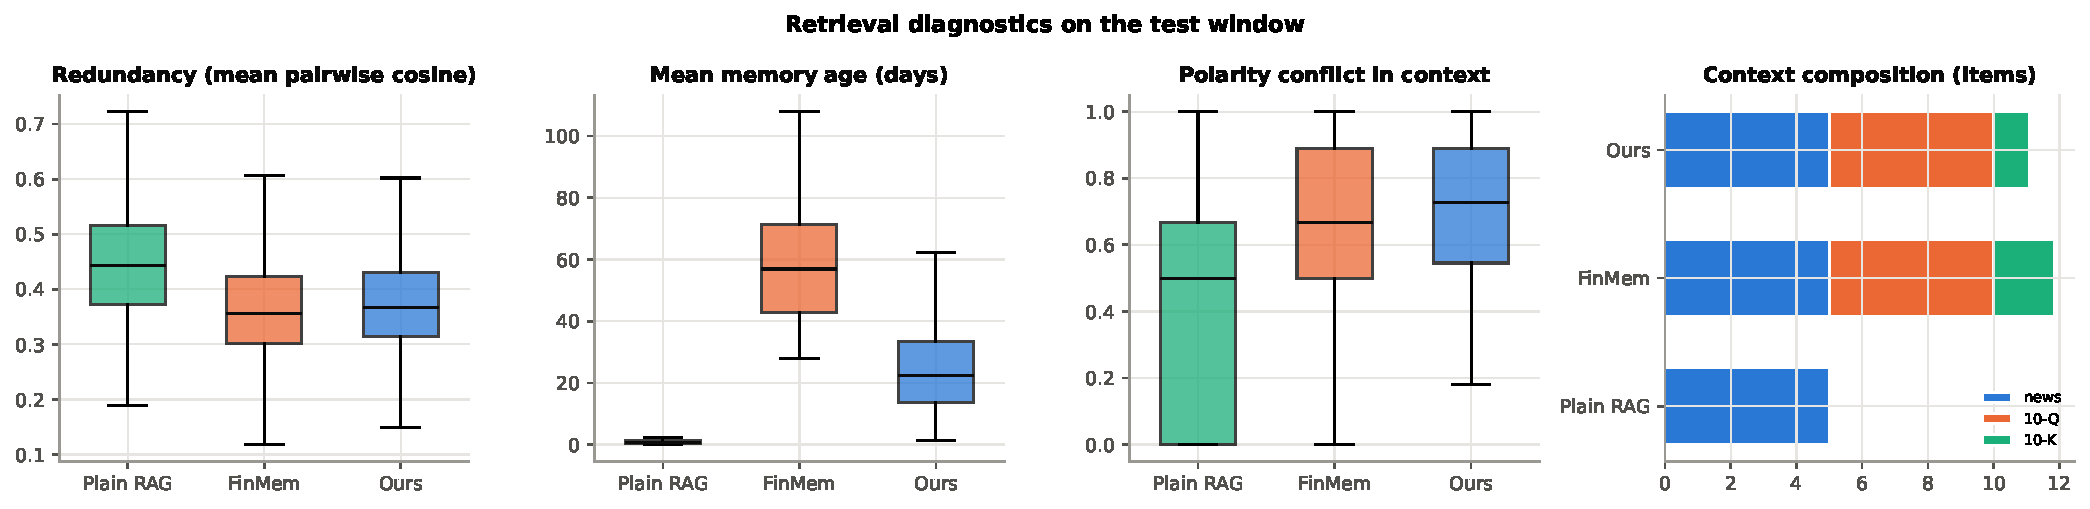
\includegraphics[width=\textwidth]{fig13_retrieval_diagnostics.pdf}
\caption{Retrieval diagnostics: redundancy, age, polarity conflict and layer composition of the retrieved context.}
\label{fig:retrieval}
\end{figure}

\begin{figure}[H]
\centering
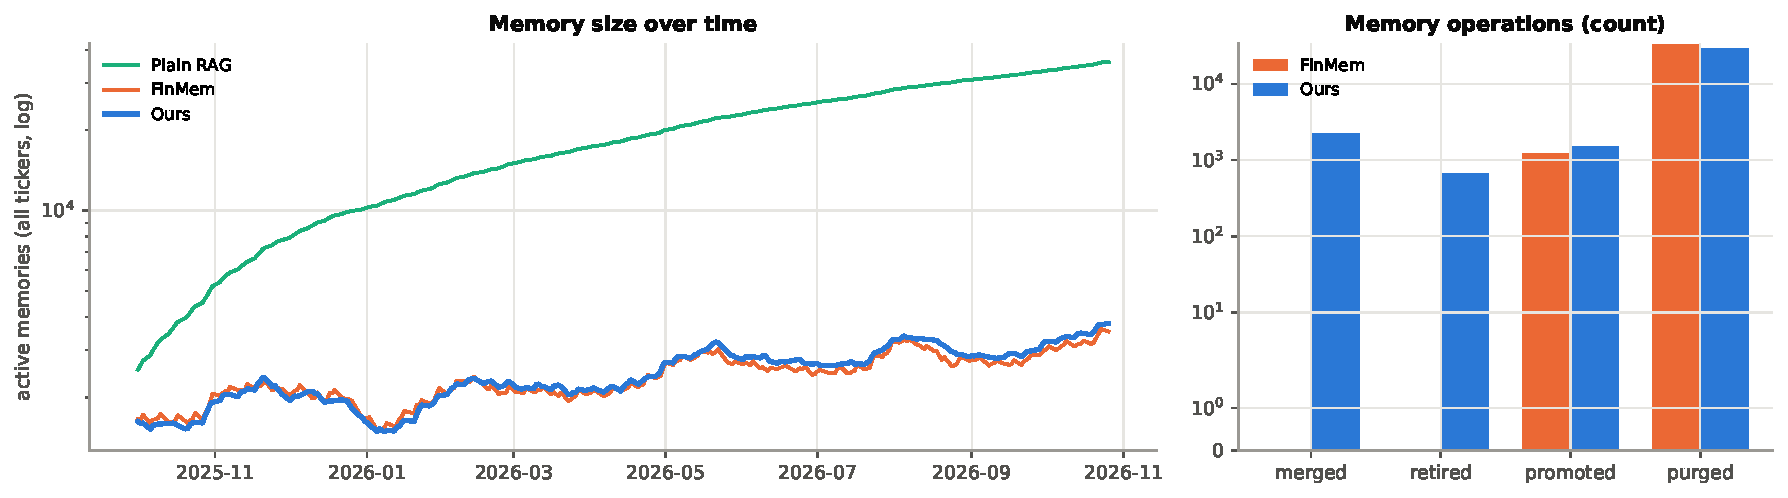
\includegraphics[width=\textwidth]{fig18_memory_dynamics.pdf}
\caption{Active memory size over time and memory operations.}
\label{fig:memdyn}
\end{figure}

\begin{figure}[H]
\centering
\begin{minipage}{0.55\textwidth}\centering
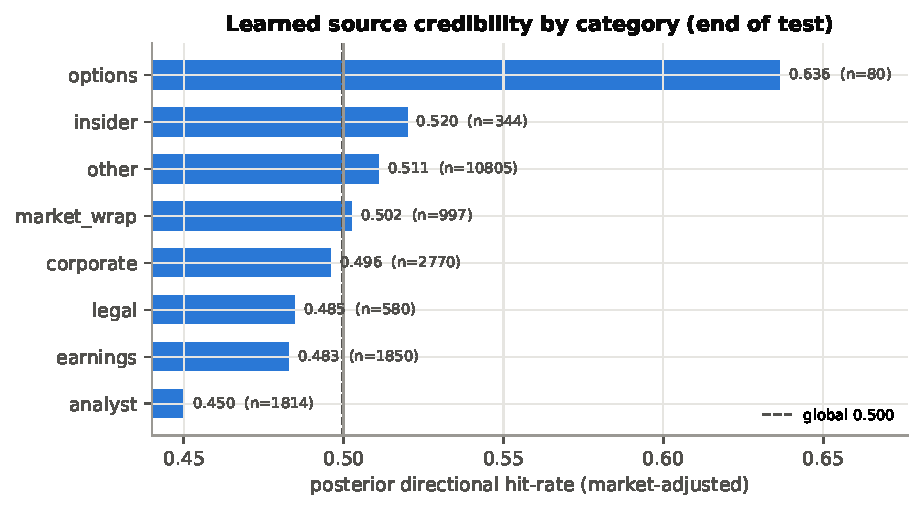
\includegraphics[width=\textwidth]{fig14_credibility.pdf}
\caption{Learned category credibility (N1).}
\label{fig:cred}
\end{minipage}\hfill
\begin{minipage}{0.42\textwidth}\centering
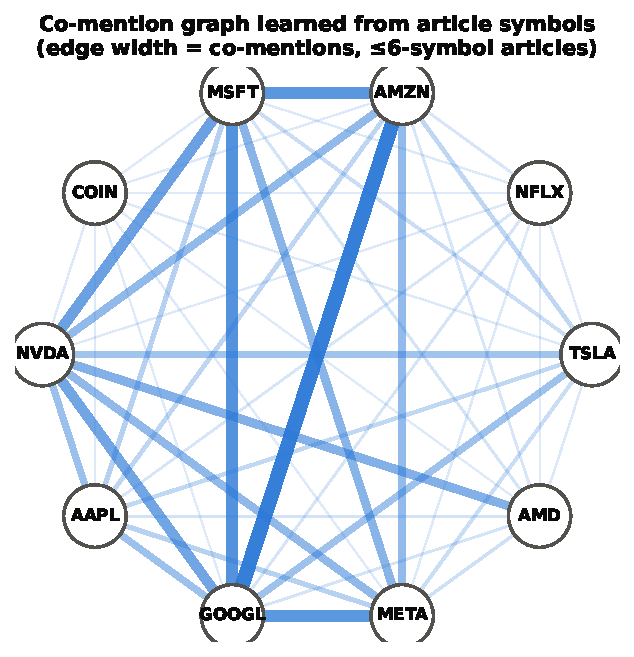
\includegraphics[width=\textwidth]{fig19_peer_graph.pdf}
\caption{Co-mention graph used by N6.}
\label{fig:peers}
\end{minipage}
\end{figure}

\subsection{LLM backbones}
Table~\ref{tab:llm} and Figure~\ref{fig:llm} report the LLM experiment: three free Groq backbones read the context retrieved by each memory (or none) for FinMem's five stocks over the last 50 test sessions (17 August -- 26 October 2026), 2{,}250 decisions in total, all parsed successfully. With every backbone, the context from our memory gives a higher return and a smaller drawdown than FinMem's context: $+2.55\%$ versus $-12.00\%$ (gpt-oss-120b), $+1.33\%$ versus $-10.70\%$ (gpt-oss-20b) and $-1.34\%$ versus $-4.79\%$ (qwen3.8-27b), with maximum drawdowns roughly halved ($-6.3/-4.8/-5.8\%$ versus $-14.7/-10.7/-10.7\%$). Pooled over backbones, the advantage over FinMem is 20.9 basis points per day but not significant (Wilcoxon $p=0.12$), and the advantage over the memory-less prompt is small and inconsistent (qwen3.8-27b does best without memory). None of the configurations clearly beats buy-and-hold over this short window ($+3.9\%$). In the action mix, our context (which includes the episodic-recall warning) makes gpt-oss-20b and qwen3.8-27b hold more often than FinMem's context (73\% and 92\% versus 61\% and 70\% Hold), while gpt-oss-120b holds equally often with both (45--46\%), so the gain is not only a matter of trading less. The three backbones agree on the same action in only 26\% of the decisions, so the choice of backbone is itself a large source of variance.

\begin{table}[ht]
\centering
\caption{LLM backbones deciding from the same retrieved memory (FinMem-style prompt, temperature 0, single trial), FinMem's five stocks, last 50 test sessions, 250 decisions per row.}
\label{tab:llm}
\small
\begin{tabular}{llrrrc}
\hline
Backbone & Memory & CR (\%) & Sharpe & MDD (\%) & Buy/Sell/Hold (\%) \\
\hline
gpt-oss-120b & No-Memory & -3.61 & -0.73 & -8.18 & 9/43/48 \\
gpt-oss-120b & FinMem & -12.00 & -3.15 & -14.74 & 28/26/46 \\
gpt-oss-120b & Ours & 2.55 & 0.74 & -6.33 & 28/27/45 \\
\hline
gpt-oss-20b & No-Memory & -6.59 & -1.74 & -7.14 & 6/56/39 \\
gpt-oss-20b & FinMem & -10.70 & -2.47 & -10.74 & 26/13/61 \\
gpt-oss-20b & Ours & 1.33 & 0.45 & -4.82 & 20/7/73 \\
\hline
qwen3.8-27b & No-Memory & 3.48 & 0.78 & -7.21 & 24/0/76 \\
qwen3.8-27b & FinMem & -4.79 & -1.15 & -10.73 & 16/13/70 \\
qwen3.8-27b & Ours & -1.34 & -0.27 & -5.77 & 6/2/92 \\
\hline
\multicolumn{6}{p{0.9\textwidth}}{\footnotesize Pooled over backbones: Ours vs FinMem: +20.9 bps/day, Wilcoxon $p=0.123$; Ours vs No-Memory: +6.1 bps/day, Wilcoxon $p=0.508$.} \\
\multicolumn{6}{p{0.9\textwidth}}{\footnotesize Buy \& Hold over the same window: CR 3.89\%.} \\
\hline
\end{tabular}
\end{table}


\begin{figure}[H]
\centering
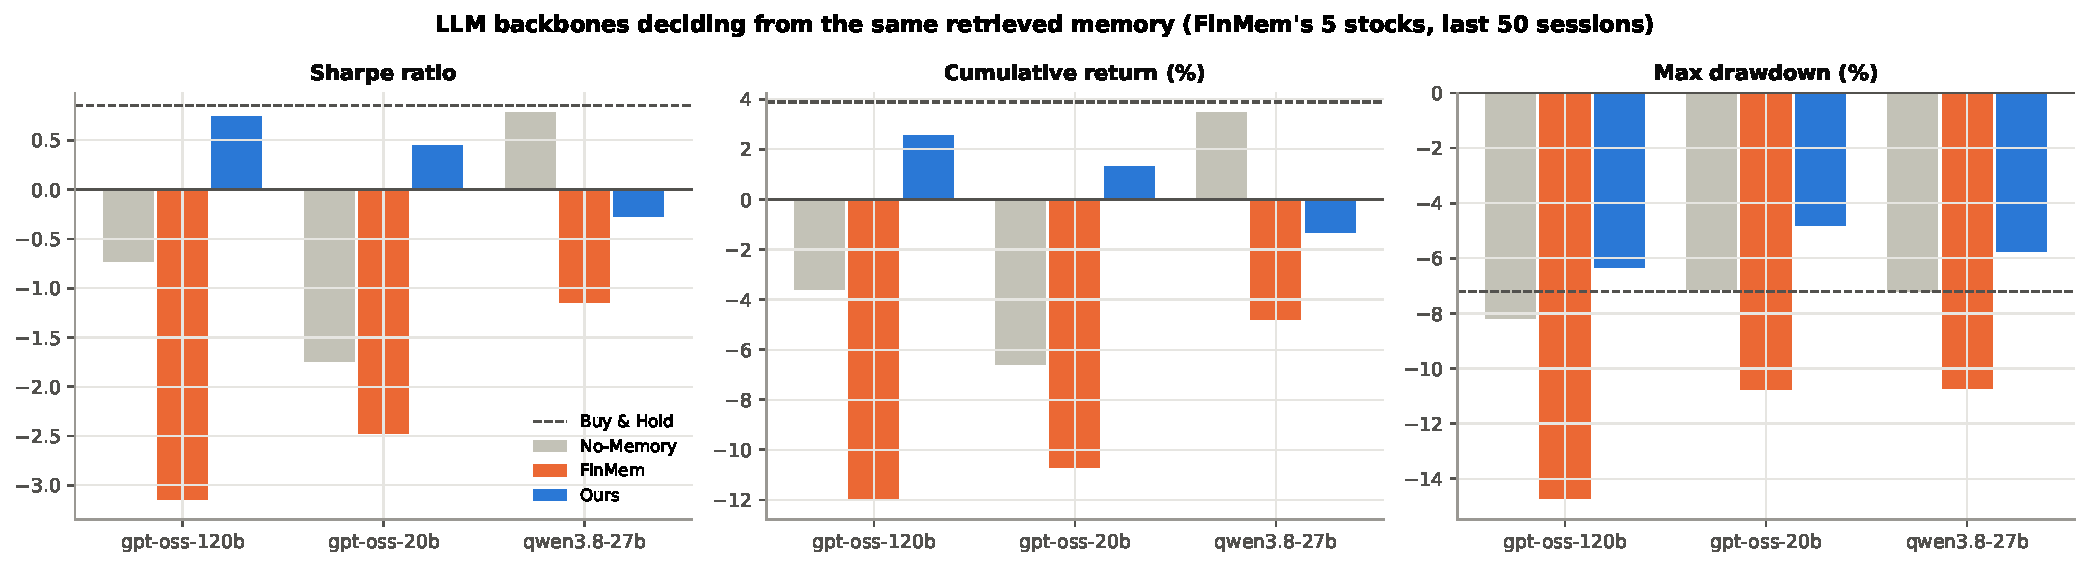
\includegraphics[width=\textwidth]{fig20_llm_backbones.pdf}
\caption{LLM backbones deciding from the same retrieved memory.}
\label{fig:llm}
\end{figure}

\section{Extension Models: Deep Learning, Reinforcement Learning and Pattern Matching}
\label{sec:ext-results}
The main study compares memory architectures with rule and gradient-boosting baselines. To test whether its conclusions depend on the model family, we evaluated five more models on exactly the same protocol (Section~\ref{sec:ext-design}): a GRU, a Transformer on price features, the same Transformer with our memory features, a tabular Q-learning agent and a nearest-neighbour pattern model, plus two exploratory combinations defined after the main results were known. The whole extension run (33 monthly network fits per model, ten Q-learning agents and ten analogue back-tests) took 531 seconds on the laptop CPU.

\subsection{Overall comparison}
Table~\ref{tab:ext-main} and Figures~\ref{fig:zoo-equity}--\ref{fig:zoo-sharpe} summarise all models. Four observations stand out.
\begin{enumerate}
  \item \textbf{A small Transformer on price features is competitive.} It earned $+11.6\%$ (Sharpe $0.95$) with the smallest drawdown of all models ($-7.9\%$), roughly on par with buy-and-hold ($+11.2\%$, $0.61$) and below the price-only LightGBM ($+19.4\%$, $1.15$). The GRU was weaker ($0.28$).
  \item \textbf{Adding news-memory features hurts learned models.} Giving the same Transformer our memory features lowered its Sharpe from $0.95$ to $0.09$ and deepened its drawdown from $-7.9\%$ to $-18.0\%$. This replicates, with a completely different model class, the main study's finding that memory features lower LightGBM's Sharpe (1.15 to 0.44). The evidence that next-day information in news memory is close to zero is therefore not specific to one model.
  \item \textbf{Reinforcement learning learned little that generalises.} The Q-learning agent earned $+4.4\%$ (Sharpe $0.39$), below buy-and-hold. It held a (long-only) position on 54\% of stock-days and its portfolio has a market beta of $0.84$, so its result largely follows the market.
  \item \textbf{The pattern model had the highest Sharpe ($1.45$), but the result is fragile} (Section~\ref{sec:analogs}): its default settings happen to be the best of nine combinations, and five of the nine are negative.
\end{enumerate}
None of these differences is statistically significant (Table~\ref{tab:ext-tests}): all 95\% bootstrap intervals for the Sharpe difference against buy-and-hold, LightGBM and our memory contain zero, and the smallest Wilcoxon $p$-value is $0.085$ (the exploratory model vote against our memory). The exploratory risk overlay, which keeps LightGBM's position but stays in cash when our memory abstains, cut LightGBM's drawdown from $-17.2\%$ to $-11.6\%$ and its volatility from 19\% to 11\% at the cost of return (Sharpe $1.03$ versus $1.15$), consistent with the earlier observation that episodic recall works more as a risk control than as a signal; because it was designed after the main results, it is a hypothesis for future work, not a finding.

\begin{table}[H]
\centering
\small
\caption{Extension models on the primary rolling protocol (10 stocks, 227 test days, 5 bps costs). Beta and alpha are against SPY; IC is the pooled Spearman correlation of the model's signal with the next-day return. $^{*}$Exploratory combinations defined after the main results were known.}
\label{tab:ext-main}
\resizebox{\textwidth}{!}{%
\begin{tabular}{lrrrrrrrr}
\toprule
Model & CR & Sharpe & Sortino & MDD & Vol & $\beta$ & $\alpha$/yr & IC \\
\midrule
Buy \& Hold & +11.2\% & +0.61 & +0.96 & -16.5\% & 24\% & +1.62 & -10.8\% & -- \\
LGBM (price) & +19.4\% & +1.15 & +1.91 & -17.2\% & 19\% & -0.11 & +23.2\% & -- \\
LogReg (price) & -21.5\% & -1.39 & -2.13 & -29.7\% & 18\% & -0.17 & -22.7\% & -- \\
GRU (price) & +3.0\% & +0.28 & +0.43 & -11.8\% & 16\% & +0.21 & +1.3\% & +0.017 \\
\textbf{Transformer (price)} & +11.6\% & +0.95 & +1.41 & -7.9\% & 14\% & -0.12 & +14.9\% & +0.024 \\
Transformer (price+memory) & +0.2\% & +0.09 & +0.15 & -18.0\% & 16\% & +0.07 & +0.5\% & +0.023 \\
\textbf{RL Q-learning} & +4.4\% & +0.39 & +0.58 & -14.7\% & 15\% & +0.84 & -7.2\% & -- \\
Pattern analogs (kNN) & +17.7\% & +1.45 & +2.15 & -6.4\% & 13\% & +0.49 & +11.2\% & +0.034 \\
\textbf{Ours} & -3.6\% & -0.20 & -0.30 & -15.2\% & 15\% & -0.33 & +2.3\% & -- \\
FinMem & -11.0\% & -0.72 & -1.03 & -19.7\% & 16\% & +0.64 & -21.7\% & -- \\
\midrule
LGBM + memory risk overlay$^{*}$ & +10.4\% & +1.03 & +1.60 & -11.6\% & 11\% & +0.06 & +10.6\% & +0.017 \\
Model vote (LGBM, Transformer, Ours)$^{*}$ & +14.9\% & +1.09 & +1.58 & -14.9\% & 15\% & -0.29 & +21.2\% & +0.036 \\
\bottomrule
\end{tabular}
}
\end{table}


\begin{figure}[H]
\centering
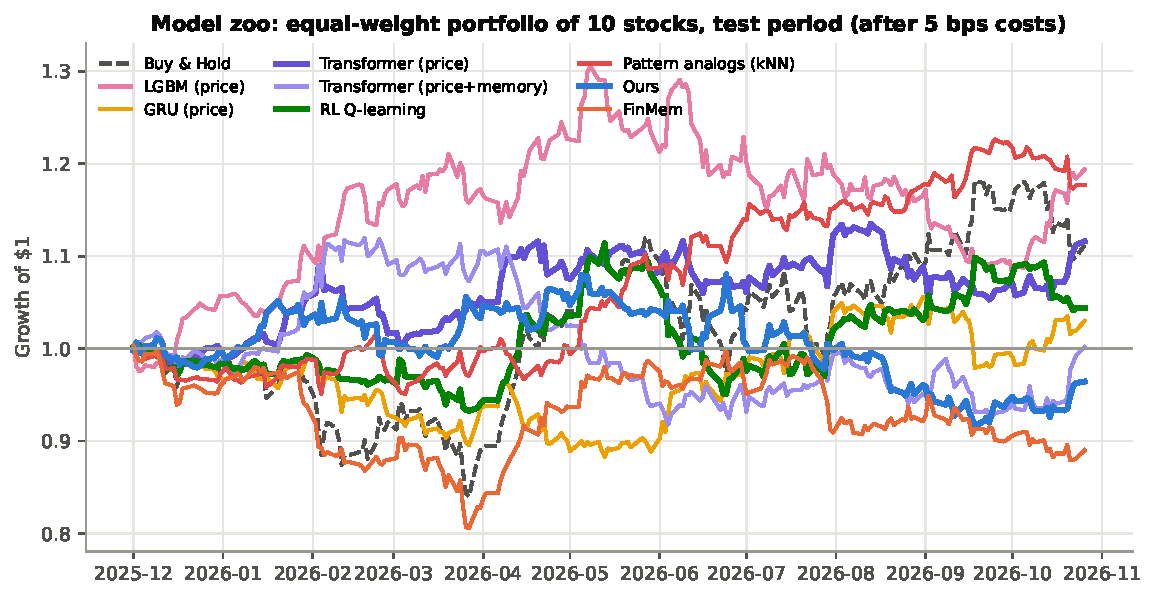
\includegraphics[width=\textwidth]{fig21_model_zoo_equity.pdf}
\caption{Growth of \$1 for all model families on the same 10-stock, 227-day test (equal weight, after costs).}
\label{fig:zoo-equity}
\end{figure}
\begin{figure}[H]
\centering
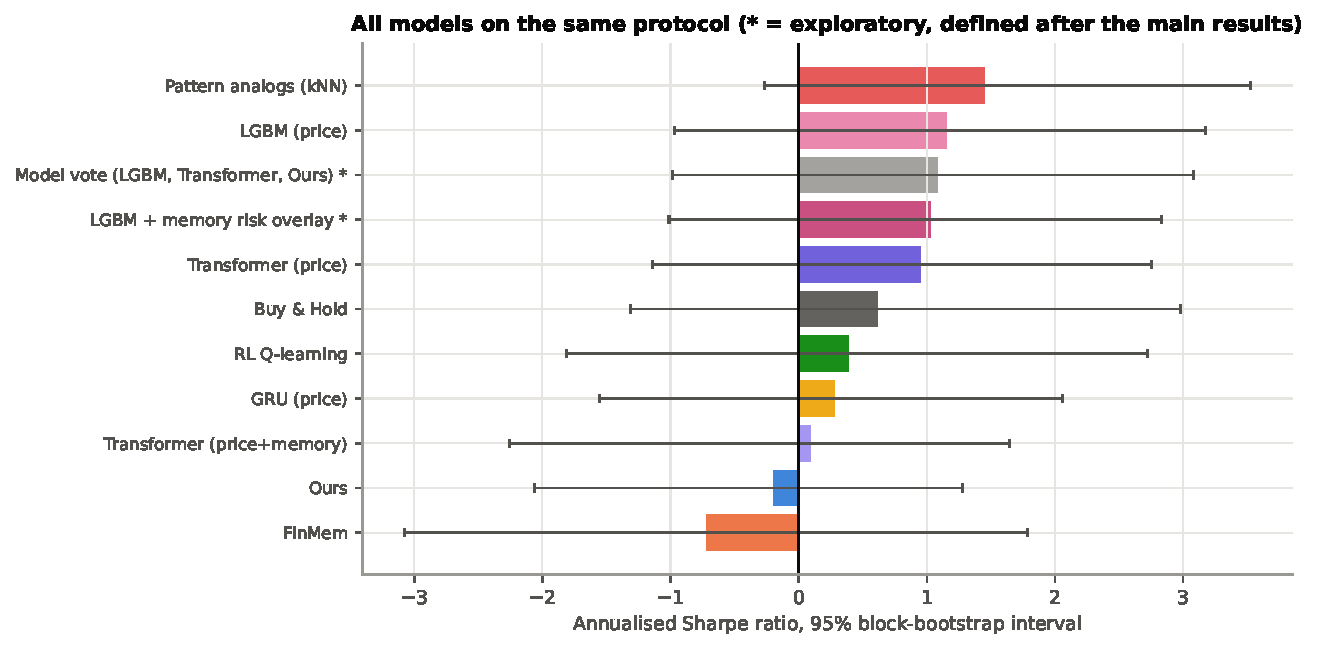
\includegraphics[width=\textwidth]{fig22_model_zoo_sharpe.pdf}
\caption{Sharpe ratio of every model with its 95\% moving-block bootstrap interval. All intervals overlap zero and each other.}
\label{fig:zoo-sharpe}
\end{figure}

\begin{figure}[!htbp]
\centering
\appshot{app_zoo_paper.png}
\caption{The same comparison in the application's Research lab.}
\label{fig:ui-zoo}
\end{figure}

\begin{table}[H]
\centering
\small
\caption{Pairwise comparisons of the extension models: $\Delta$Sharpe with 95\% block-bootstrap interval and Wilcoxon signed-rank $p$ on daily portfolio returns, against buy-and-hold, the price-only LightGBM and our memory.}
\label{tab:ext-tests}
\resizebox{\textwidth}{!}{%
\begin{tabular}{lrrrrrr}
\toprule
Model & \multicolumn{2}{c}{vs Buy \& Hold} & \multicolumn{2}{c}{vs LGBM (price)} & \multicolumn{2}{c}{vs Ours} \\
 & $\Delta$Sharpe [CI] & $p$ & $\Delta$Sharpe [CI] & $p$ & $\Delta$Sharpe [CI] & $p$ \\
\midrule
GRU (price) & -0.33 [-3.5, +2.5] & 0.72 & -0.87 [-3.7, +1.9] & 0.71 & +0.48 [-1.9, +3.2] & 0.58 \\
Transformer (price) & +0.34 [-2.7, +3.0] & 0.73 & -0.20 [-2.8, +2.1] & 0.82 & +1.15 [-0.9, +3.2] & 0.12 \\
Transformer (price+memory) & -0.52 [-4.7, +2.5] & 0.78 & -1.06 [-4.2, +1.2] & 0.95 & +0.29 [-2.3, +2.4] & 0.58 \\
RL Q-learning & -0.22 [-1.4, +1.0] & 0.49 & -0.76 [-3.7, +2.4] & 0.41 & +0.58 [-2.0, +3.8] & 0.77 \\
Pattern analogs (kNN) & +0.84 [-2.0, +3.3] & 0.50 & +0.30 [-2.7, +3.7] & 0.78 & +1.65 [-0.4, +4.5] & 0.24 \\
LGBM + memory risk overlay$^{*}$ & +0.42 [-2.9, +3.1] & 0.82 & -0.12 [-1.5, +1.2] & 0.41 & +1.23 [-1.2, +3.9] & 0.59 \\
Model vote (LGBM, Transformer, Ours)$^{*}$ & +0.48 [-2.9, +3.3] & 0.82 & -0.06 [-2.0, +1.6] & 0.98 & +1.28 [-0.4, +3.1] & 0.09 \\
\bottomrule
\end{tabular}
}
\end{table}


\subsection{What the neural networks learned}
Figure~\ref{fig:deep-training} looks inside the networks. On the held-out last 15\% of each training set, the validation loss never fell clearly below that of a coin flip ($\ln 2 = 0.693$): the best validation losses averaged $0.683$ (GRU), $0.689$ (Transformer) and $0.693$ (Transformer with memory), and early stopping chose epoch 7 on average for the Transformer. The training loss of the memory-augmented Transformer fell much faster than that of the price-only one while its validation loss rose, the signature of over-fitting to extra features that do not generalise. The attention of the decision day over the 20-day window is almost uniform (the dotted line marks $1/20$); the price-only Transformer puts slightly more weight on the most recent five days (25.6\% versus 24.8\% on the oldest five). In short, the networks found only a faint next-day signal, and their trading results should be read with that in mind.

\begin{figure}[H]
\centering
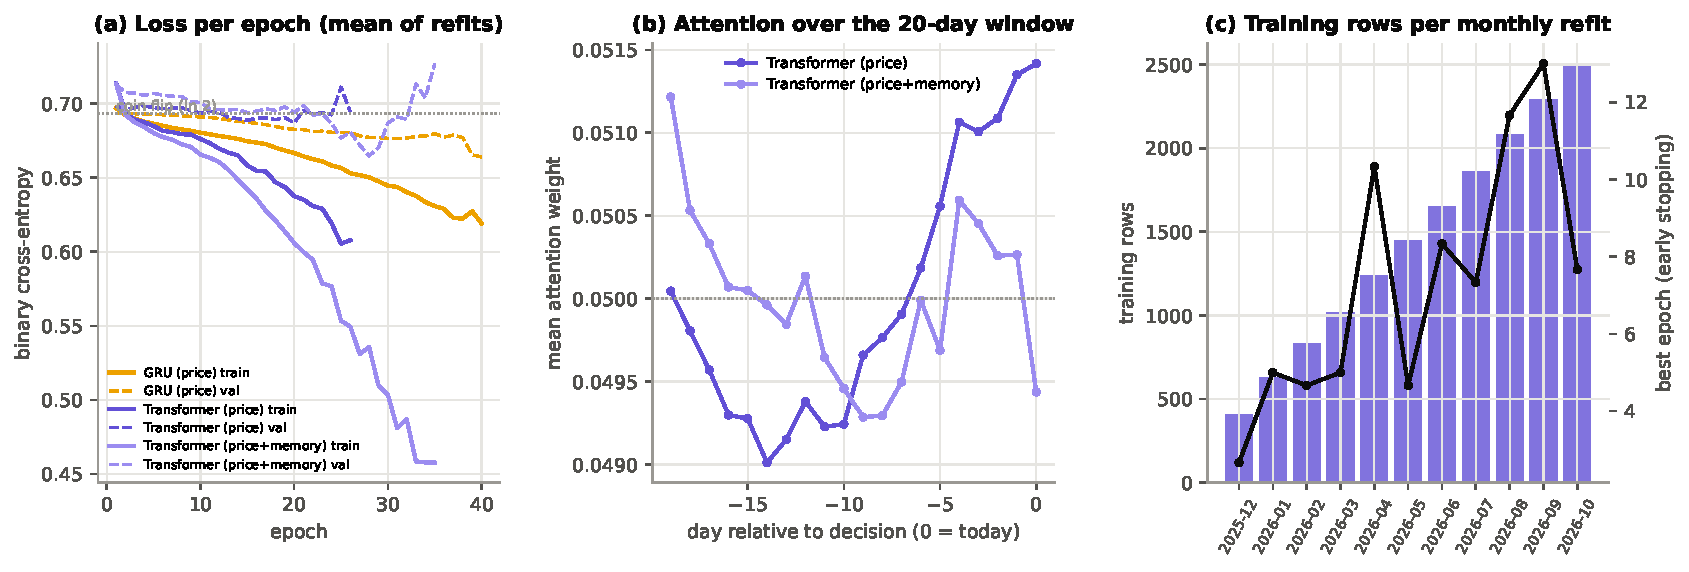
\includegraphics[width=\textwidth]{fig23_deep_training.pdf}
\caption{Deep models: (a) training and validation loss per epoch averaged over refits; (b) attention of the decision day over the 20-day window; (c) size of the training set at each monthly refit and the epoch chosen by early stopping.}
\label{fig:deep-training}
\end{figure}

\subsection{Reinforcement-learning agent}
Figure~\ref{fig:rl} shows the Q-learning agent. Its pre-training reward per decision fluctuates between passes instead of rising steadily, because each pass explores differently and daily rewards are dominated by noise. After 30 passes and the online updates of the test window, the agent had learned from 42{,}320 transitions and visited 25 of the 36 possible situations. Per stock it beat buy-and-hold on four stocks, AAPL (Sharpe $2.03$ versus $1.05$), AMD ($2.09$ versus $1.86$), MSFT and COIN, and lost on the other six, most clearly on NVDA, GOOGL and TSLA (Table~\ref{tab:ext-per-ticker}). The learned policy (panel c) is mostly ``stay invested'', with a strong exception: when the stock has fallen over five days, is below its 20-day average and RSI is neutral, the agent prefers to sell what it holds. The application exposes the same agent per stock, with its Q-table, its decision log and the reward of every decision (Figure~\ref{fig:ui-rl}).

\begin{figure}[H]
\centering
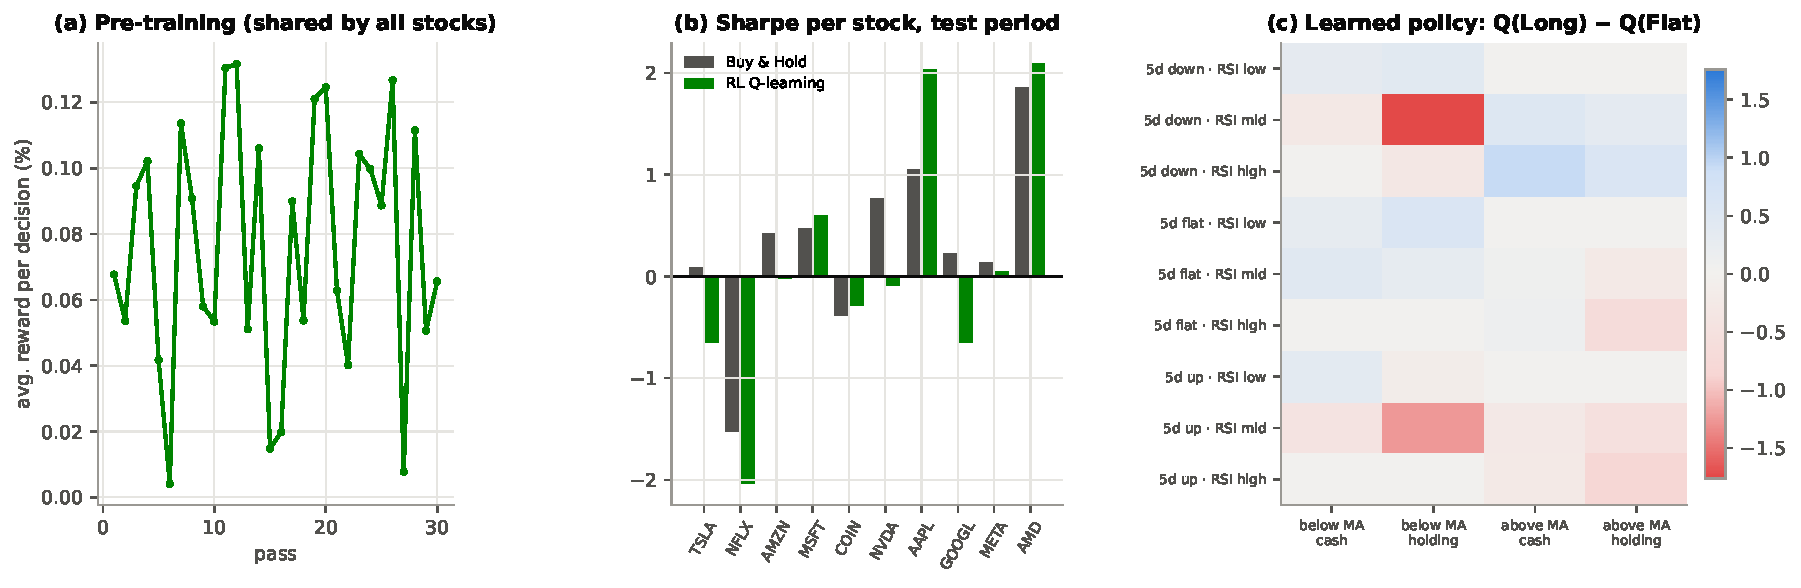
\includegraphics[width=\textwidth]{fig24_rl_agent.pdf}
\caption{Q-learning agent: (a) average reward per decision in each pre-training pass; (b) Sharpe ratio per stock against buy-and-hold in the test period; (c) learned preference for holding over cash, $Q(\text{Long})-Q(\text{Flat})$, in each market situation (averaged over the ten stock-specific agents).}
\label{fig:rl}
\end{figure}

\begin{table}[H]
\centering
\small
\caption{Sharpe ratio per stock in the test period.}
\label{tab:ext-per-ticker}
\resizebox{\textwidth}{!}{%
\begin{tabular}{lrrrrrrrrrr}
\toprule
Model & TSLA & NFLX & AMZN & MSFT & COIN & NVDA & AAPL & GOOGL & META & AMD \\
\midrule
Buy \& Hold & +0.09 & -1.52 & +0.42 & +0.47 & -0.38 & +0.77 & +1.05 & +0.23 & +0.13 & +1.86 \\
LGBM & +1.38 & -0.06 & +0.69 & -1.22 & +0.68 & +2.13 & -0.92 & +0.57 & +0.18 & +0.63 \\
GRU & -0.72 & +0.03 & +1.21 & -0.90 & +0.42 & +1.16 & +0.02 & -0.28 & +0.54 & -0.28 \\
Transf. & +0.69 & +0.50 & +0.02 & +0.53 & +0.23 & +0.36 & +0.18 & -0.10 & +0.52 & +0.16 \\
Transf.+mem & -0.79 & +1.08 & -0.65 & -1.43 & +0.36 & +1.47 & -0.91 & -0.48 & +2.20 & -0.77 \\
RL Q-learning & -0.65 & -2.04 & -0.02 & +0.59 & -0.28 & -0.09 & +2.03 & -0.65 & +0.05 & +2.09 \\
Analogs & -2.29 & +0.82 & +0.75 & -0.10 & +1.26 & +0.96 & +0.35 & +0.22 & +0.82 & +1.13 \\
Ours & -1.39 & +2.33 & -0.52 & +0.64 & +0.08 & -0.64 & +0.66 & +0.27 & -1.66 & +0.12 \\
FinMem & -0.99 & +0.26 & -0.54 & +0.05 & -1.73 & +0.84 & +0.56 & -1.61 & +0.09 & +0.86 \\
\bottomrule
\end{tabular}
}
\end{table}


\subsection{Pattern analogues}
\label{sec:analogs}
Figure~\ref{fig:analogs} repeats the pattern model for every combination of pattern length (10, 20, 40 days) and look-ahead (5, 10, 20 days) on a common test period. Averaged over the ten stocks, five of the nine settings have a negative Sharpe ratio, two more are close to zero (0.01 and 0.04), and only one setting, the 20-day pattern with a 10-day look-ahead (0.50), beats the average buy-and-hold Sharpe ratio of 0.35; even that setting beats buy-and-hold on just 6 of 10 stocks. The default (20-day pattern, 10-day look-ahead, chosen for the application before any test) happens to be the best cell. We therefore do not claim that chart patterns predict returns: the strong portfolio result of Table~\ref{tab:ext-main} is the kind of outcome that the multiple-testing literature~\cite{harvey2016cross,bailey2014deflated} warns about. For a single stock the picture can be much worse; on TSLA alone the same settings lost $50\%$, and the forecasts were negatively correlated with what happened next (Figure~\ref{fig:ui-pattern}).

\begin{figure}[H]
\centering
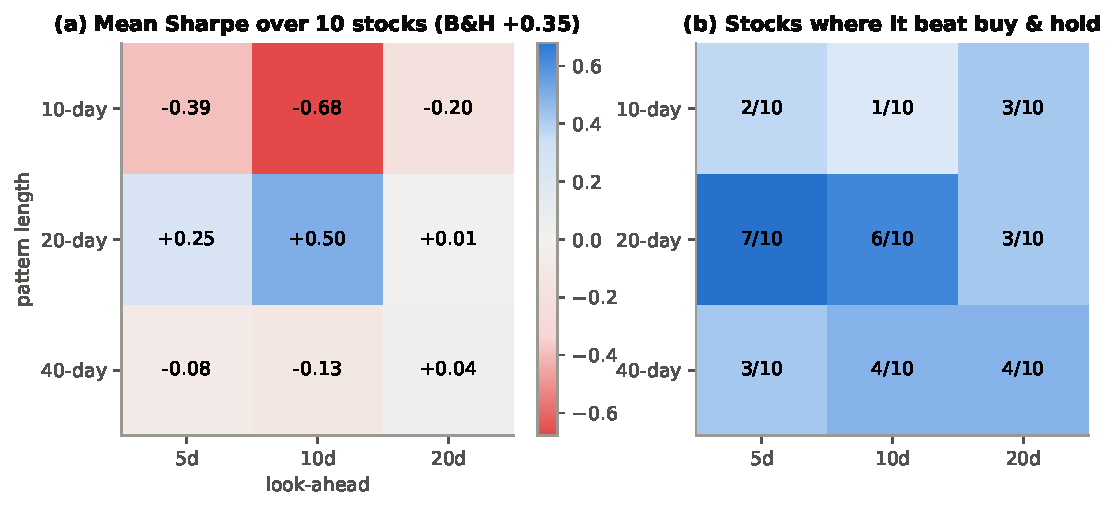
\includegraphics[width=\textwidth]{fig25_pattern_analogs.pdf}
\caption{Robustness of the pattern model: (a) mean Sharpe over the ten stocks for every pattern length and look-ahead, compared with buy-and-hold; (b) number of stocks on which each setting beat buy-and-hold.}
\label{fig:analogs}
\end{figure}
\begin{figure}[!htbp]
\centering
\appshot{app_pattern_paper_1.png}
\caption{Pattern finder in the application (TSLA): the latest 20-day pattern (bold) against the most similar past windows and what followed, the verdict, the daily back-test against buy-and-hold and the robustness grid.}
\label{fig:ui-pattern}
\end{figure}
\begin{figure}[!htbp]
\ContinuedFloat
\centering
\appshot{app_pattern_paper_2.png}
\caption[]{(continued)}
\end{figure}

\section{Portfolio Construction}
\label{sec:alloc-results}
The application advises how to split a budget across stocks (Section~\ref{sec:autopilot-design}). Table~\ref{tab:ext-alloc} and Figure~\ref{fig:alloc} compare the methods walk-forward: every 21 trading days the weights are recomputed from the previous 120 days only, with 80\% of the budget invested and at most 25\% per stock. Equal weight ($+10.7\%$, Sharpe $0.77$) and risk parity ($+9.2\%$, $0.75$) did better than minimum variance ($+5.1\%$, $0.51$), which concentrated in a few calm stocks (up to the 25\% cap in AAPL); all three had similar drawdowns of about $-12\%$. This matches the classic out-of-sample result that naive diversification is hard to beat~\cite{demiguel2009naive}. Investing the same 80\% in the S\&P 500 was the best risk-adjusted choice ($+10.0\%$, Sharpe $1.26$, drawdown $-7.1\%$): the ten technology-heavy stocks are highly correlated (Figure~\ref{fig:market-risk}), so splitting money among them diversifies less than holding the broad market. The application shows these numbers next to its suggestion so that the user sees this trade-off.

\begin{table}[H]
\centering
\small
\caption{Budget-split (portfolio construction) methods, walk-forward with monthly rebalancing, 80\% invested, at most 25\% of the budget per stock. SPY row: the same 80\% invested in the S\&P 500.}
\label{tab:ext-alloc}
\begin{tabular}{lrrrr}
\toprule
Method & Return & Volatility & Sharpe & MDD \\
\midrule
Risk parity (inverse volatility) & +9.2\% & 18\% & +0.75 & -11.7\% \\
Minimum variance & +5.1\% & 15\% & +0.51 & -11.6\% \\
Equal weight & +10.7\% & 20\% & +0.77 & -12.1\% \\
SPY (same exposure) & +10.0\% & 10\% & +1.26 & -7.1\% \\
\bottomrule
\end{tabular}
\end{table}


\begin{figure}[H]
\centering
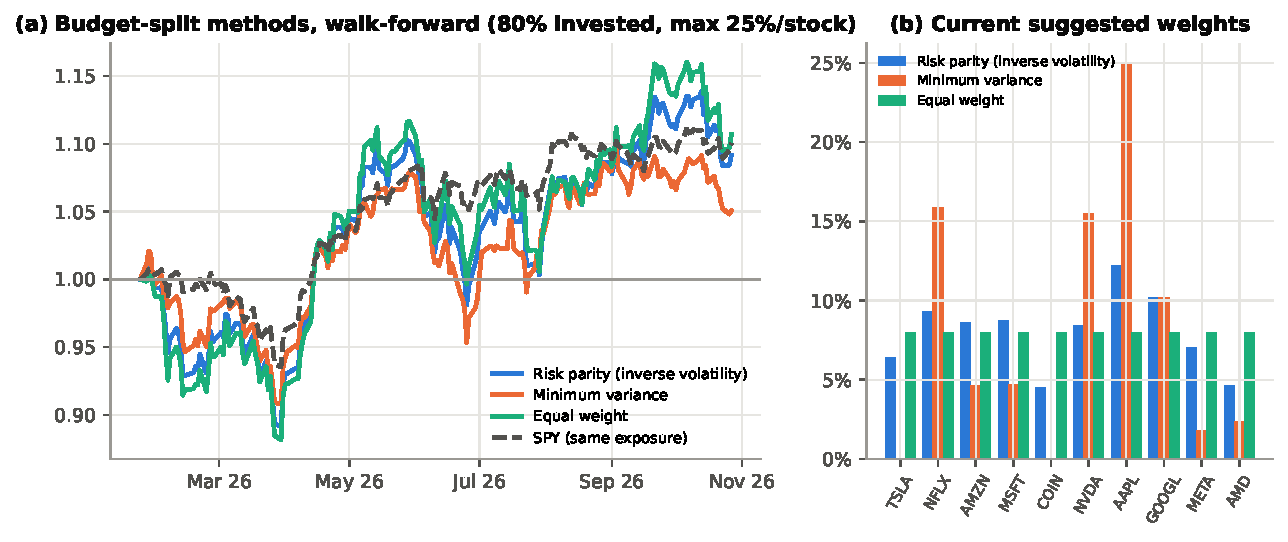
\includegraphics[width=\textwidth]{fig26_allocation.pdf}
\caption{Budget-split methods: (a) walk-forward growth with monthly rebalancing; (b) weights each method suggests today.}
\label{fig:alloc}
\end{figure}
\begin{figure}[!htbp]
\centering
\appshot{app_split_paper_1.png}
\caption{Budget split in the application: method choice, suggested amounts per stock with the trades needed to reach them, plan statistics and the walk-forward comparison.}
\label{fig:ui-split}
\end{figure}
\begin{figure}[!htbp]
\ContinuedFloat
\centering
\appshot{app_split_paper_2.png}
\caption[]{(continued)}
\end{figure}

\section{Robustness and Statistical Power}
\label{sec:robust}

\subsection{Market exposure (CAPM)}
Raw returns mix skill with market exposure. Table~\ref{tab:ext-capm} and Figure~\ref{fig:capm} decompose every strategy's daily portfolio return into a market beta and an annualised alpha against the S\&P 500. The equal-weight basket of our ten stocks has a beta of $1.62$: buy-and-hold is a leveraged bet on the market and its alpha is negative ($-10.8\%$). Our memory has a \emph{negative} beta ($-0.33$, because it is short 58\% of the time) and a small positive alpha ($+2.3\%$), whereas FinMem has a positive beta ($0.64$) and a clearly negative alpha ($-21.7\%$). In a year in which the market rose, a negative beta explains most of the gap between our memory and buy-and-hold. The largest alphas belong to the price-only LightGBM ($+23.2\%$, $t=1.18$), the Transformer ($+14.9\%$, $t=1.03$) and the pattern model ($+11.2\%$); none is statistically significant ($|t|<2$).

\begin{table}[H]
\centering
\small
\caption{CAPM decomposition of daily portfolio returns against SPY: market beta, annualised alpha and its $t$-statistic.}
\label{tab:ext-capm}
\begin{tabular}{lrrr}
\toprule
Strategy & $\beta$ & $\alpha$ per year & $t(\alpha)$ \\
\midrule
Buy \& Hold & +1.62 & -10.8\% & -0.82 \\
LGBM (price) & -0.11 & +23.2\% & +1.18 \\
LogReg (price) & -0.17 & -22.7\% & -1.18 \\
Ours & -0.33 & +2.3\% & +0.15 \\
FinMem & +0.64 & -21.7\% & -1.47 \\
Plain RAG & +0.18 & -12.7\% & -0.80 \\
GRU (price) & +0.21 & +1.3\% & +0.08 \\
Transformer (price) & -0.12 & +14.9\% & +1.03 \\
Transformer (price+memory) & +0.07 & +0.5\% & +0.03 \\
RL Q-learning & +0.84 & -7.2\% & -0.61 \\
Pattern analogs (kNN) & +0.49 & +11.2\% & +0.92 \\
Momentum (1d) & -0.02 & -10.0\% & -0.54 \\
MA-Crossover & -0.23 & +1.4\% & +0.07 \\
Mean-Reversion (5d) & +0.19 & -6.7\% & -0.37 \\
\bottomrule
\end{tabular}
\end{table}


\begin{figure}[H]
\centering
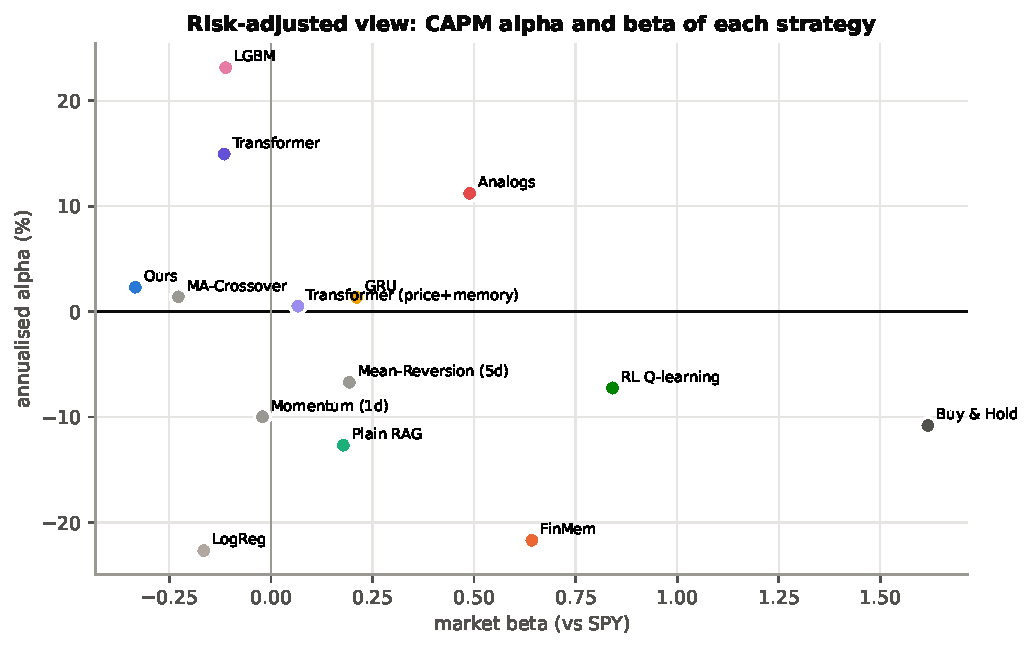
\includegraphics[width=0.85\textwidth]{fig27_capm_alpha_beta.pdf}
\caption{Market beta and annualised CAPM alpha of every strategy against the S\&P 500.}
\label{fig:capm}
\end{figure}

\subsection{Does Tesla drive the result?}
Tesla fell $5.3\%$ over the test window and was the stock on which our memory did worst (Sharpe $-1.39$). Table~\ref{tab:ext-robust} and Figure~\ref{fig:robust} recompute the portfolio without it. Our memory improves from $-0.20$ to $+0.23$ and FinMem from $-0.72$ to $-0.43$, but the ranking does not change: buy-and-hold ($0.67$), LightGBM ($0.92$) and the Transformer ($0.79$) remain ahead. Leaving out each stock in turn, our memory beats FinMem in 9 of 10 cases (the exception is leaving out COIN), and the Sharpe advantage ranges from $-0.34$ to $+1.11$ around the full-sample $+0.52$. The comparison between memories is therefore not an artefact of one stock, while the conclusion that news memory does not beat buy-and-hold also holds without Tesla. Choosing the end of the test period by waiting for any stock to recover would bias the evaluation and was deliberately avoided.

\begin{table}[H]
\centering
\small
\caption{Robustness to the stock set: Sharpe with all ten stocks, without Tesla, and on FinMem's five stocks.}
\label{tab:ext-robust}
\begin{tabular}{lrrr}
\toprule
Model & 10 stocks & without TSLA & FinMem's 5 \\
\midrule
Buy \& Hold & +0.61 & +0.67 & -0.34 \\
LGBM (price) & +1.15 & +0.92 & +0.74 \\
Ours & -0.20 & +0.23 & +0.28 \\
FinMem & -0.72 & -0.43 & -1.59 \\
Plain RAG & -0.65 & -0.10 & -1.59 \\
Transformer (price) & +0.95 & +0.79 & +0.77 \\
RL Q-learning & +0.39 & +0.59 & -0.77 \\
\bottomrule
\end{tabular}
\end{table}


\begin{figure}[H]
\centering
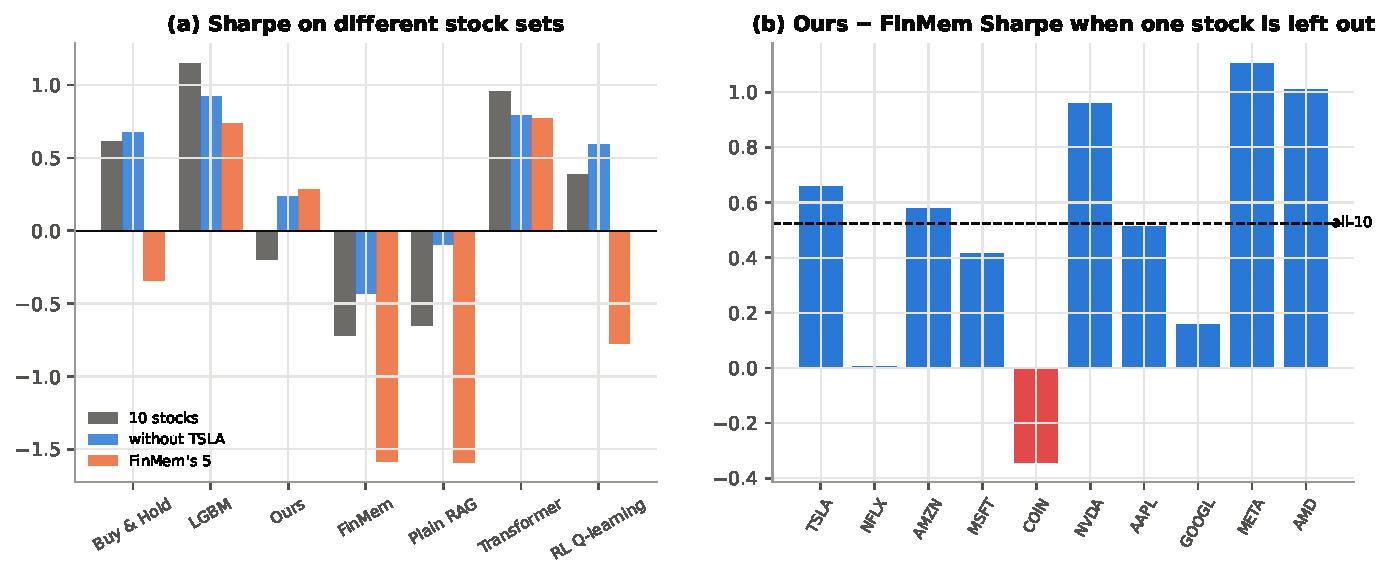
\includegraphics[width=\textwidth]{fig28_robustness.pdf}
\caption{Robustness: (a) Sharpe ratio on all ten stocks, without Tesla and on FinMem's five stocks; (b) Sharpe advantage of our memory over FinMem when one stock is left out (dashed line: all ten stocks).}
\label{fig:robust}
\end{figure}

\subsection{Market regimes}
Table~\ref{tab:ext-regimes} and Figure~\ref{fig:regimes} split the test days by whether the S\&P 500 rose (117 days) or fell (110 days). Buy-and-hold gains about 100 basis points on up days and loses about 95 on down days. Our memory and the Transformer behave in the opposite way, losing slightly on up days and gaining 16--19 basis points on down days, and LightGBM gains a little on both (6 and 11 basis points); FinMem and the Q-learning agent follow the market. Models that hedge market falls are attractive as diversifiers, but over a rising year they lag buy-and-hold.

\begin{table}[H]
\centering
\small
\caption{Average daily result (basis points) on days when the S\&P 500 rose versus fell.}
\label{tab:ext-regimes}
\begin{tabular}{lrr}
\toprule
Strategy & up days & down days \\
\midrule
Buy \& Hold & +100.2 & -94.6 \\
LGBM (price) & +6.2 & +11.0 \\
Ours & -17.2 & +15.9 \\
FinMem & +35.8 & -47.6 \\
Plain RAG & +8.5 & -17.1 \\
Transformer (price) & -8.0 & +19.3 \\
RL Q-learning & +53.8 & -52.3 \\
Pattern analogs (kNN) & +32.2 & -18.7 \\
\bottomrule
\end{tabular}
\end{table}


\begin{figure}[H]
\centering
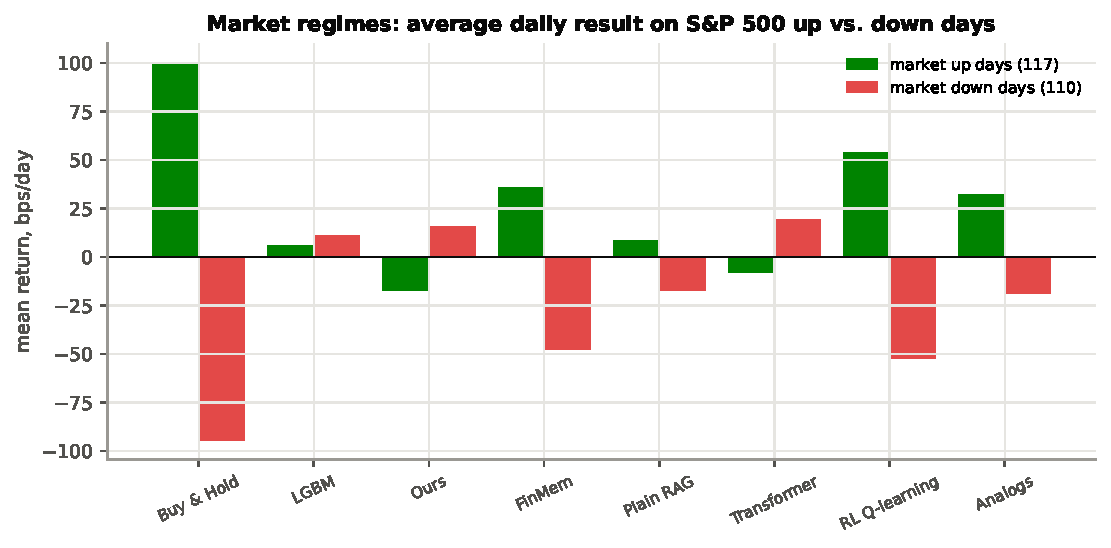
\includegraphics[width=\textwidth]{fig30_regimes.pdf}
\caption{Average daily result on days when the S\&P 500 rose versus fell.}
\label{fig:regimes}
\end{figure}
\begin{figure}[H]
\centering
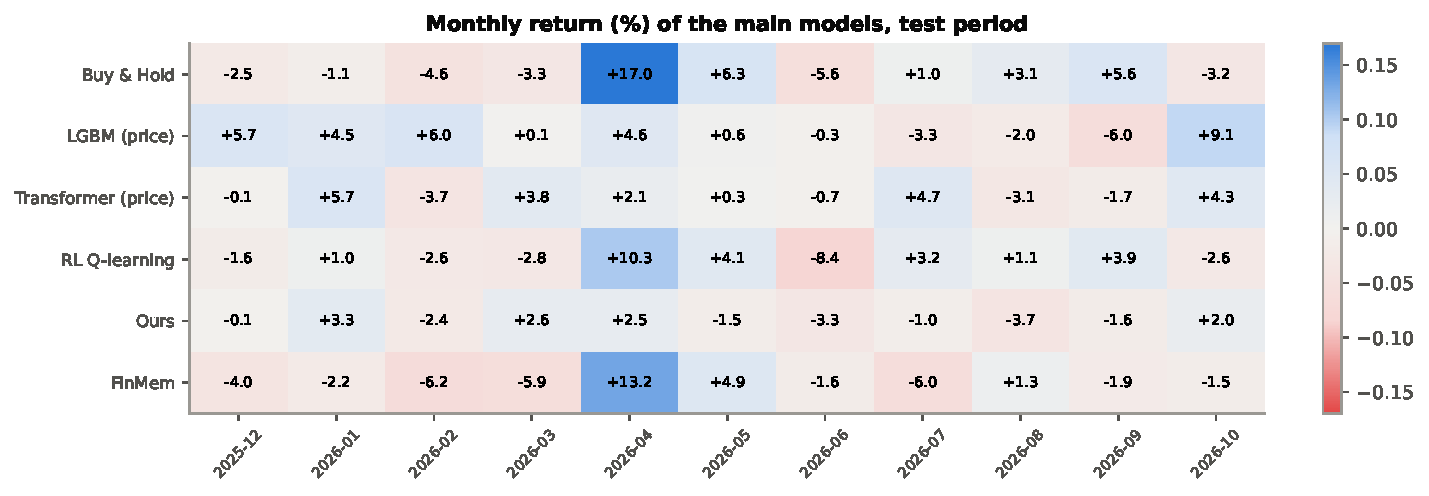
\includegraphics[width=\textwidth]{fig32_monthly_models.pdf}
\caption{Monthly returns of the main models in the test period.}
\label{fig:monthly-models}
\end{figure}

\subsection{Statistical power}
How much data would we need to prove that our memory beats FinMem? The daily difference between the two portfolios averages $\powerMean$ basis points with a standard deviation of $\powerSd$ basis points. With $\powerN$ days, a two-sided test at the 5\% level has 80\% power only for differences of at least $\powerMde$ basis points per day, seven times larger than the observed one. Detecting the observed edge with 80\% power would need about $\powerNeed$ trading days, roughly $\powerYears$ years (Figure~\ref{fig:power}). No realistic extension of the test period, and certainly not waiting a few weeks for a stock to recover, can turn this comparison into a significant result. The honest conclusion is that the memory comparison is \emph{directionally consistent} (positive in 9 of 10 leave-one-out cases, on FinMem's own stocks and with every LLM backbone) but \emph{statistically inconclusive}.

\begin{figure}[H]
\centering
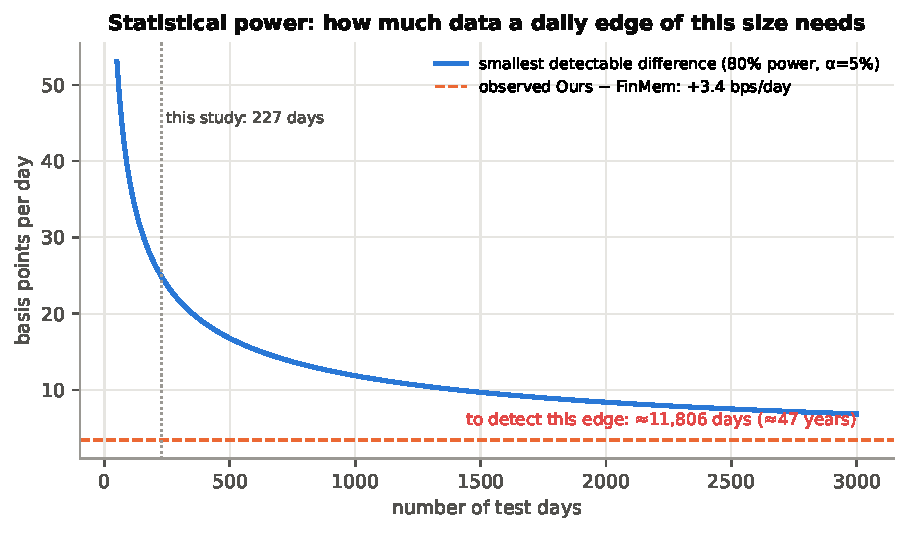
\includegraphics[width=0.85\textwidth]{fig29_power.pdf}
\caption{Smallest daily return difference detectable with 80\% power as a function of the number of test days, compared with the observed difference between our memory and FinMem.}
\label{fig:power}
\end{figure}

\subsection{Risk profile of the universe}
Table~\ref{tab:ext-stock-risk} and Figure~\ref{fig:market-risk} describe the stocks themselves. Annualised volatility ranges from 25\% (AAPL) to 69\% (COIN and AMD); COIN fell 64\% from its peak. The pairwise correlations are moderate (mostly 0.1--0.5), while the stocks' correlations with the S\&P 500 and Nasdaq-100 reach 0.6--0.7, so a large part of every stock's movement is common market risk. These numbers also explain why risk-parity weights favour AAPL and MSFT and give little to COIN and AMD.

\begin{table}[H]
\centering
\small
\caption{Risk profile of each stock over the full price history (Aug 2025 -- Oct 2026).}
\label{tab:ext-stock-risk}
\resizebox{\textwidth}{!}{%
\begin{tabular}{lrrrrrrr}
\toprule
Stock & Vol/yr & MDD & VaR$_{95}$ & CVaR$_{95}$ & $\beta$ & Skew & Ex.\ kurt. \\
\midrule
TSLA & 45\% & -39.1\% & 4.3\% & 5.9\% & 2.27 & -0.29 & 1.82 \\
NFLX & 35\% & -50.5\% & 3.4\% & 5.2\% & 0.29 & +0.17 & 6.95 \\
AMZN & 33\% & -21.7\% & 3.0\% & 4.0\% & 1.46 & +1.49 & 9.58 \\
MSFT & 30\% & -34.5\% & 2.7\% & 3.8\% & 0.99 & +1.35 & 15.55 \\
COIN & 69\% & -63.6\% & 6.5\% & 8.2\% & 2.93 & +0.53 & 1.11 \\
NVDA & 36\% & -20.2\% & 3.7\% & 4.5\% & 1.91 & +0.17 & 0.67 \\
AAPL & 25\% & -13.8\% & 2.0\% & 3.4\% & 0.69 & -0.24 & 3.06 \\
GOOGL & 31\% & -21.2\% & 2.5\% & 3.7\% & 1.38 & +0.77 & 3.78 \\
META & 40\% & -33.3\% & 3.5\% & 5.7\% & 1.48 & +0.21 & 4.39 \\
AMD & 69\% & -27.8\% & 5.9\% & 8.0\% & 3.13 & +0.73 & 4.00 \\
\bottomrule
\end{tabular}
}
\end{table}


\begin{figure}[H]
\centering
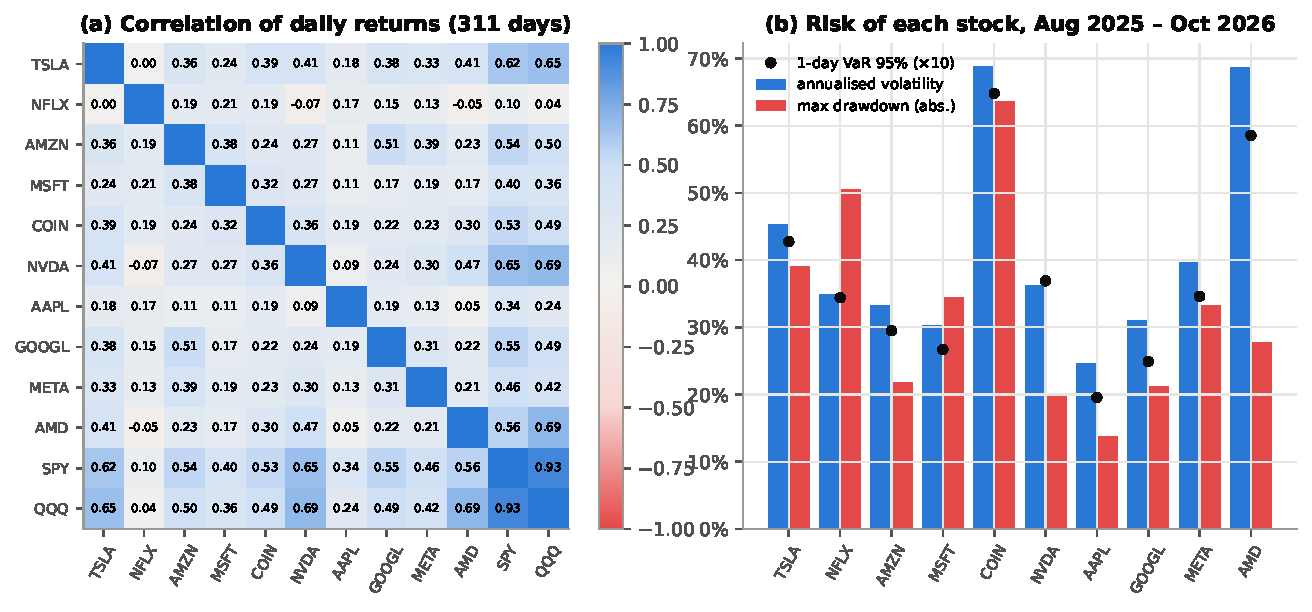
\includegraphics[width=\textwidth]{fig31_market_risk.pdf}
\caption{Market structure: (a) correlation of daily returns over the full history; (b) volatility, maximum drawdown and one-day 95\% value-at-risk of each stock.}
\label{fig:market-risk}
\end{figure}

\section{The Application}
\label{sec:app-results}
The application operationalises these findings. Because no single signal is reliable, its default recommendation is a conservative consensus: the memory action and the price-model vote must not disagree, the price model votes only when $|P(\text{up})-0.5|\ge 0.03$, episodic abstention forces Hold, and confidence is capped at 0.6. The LLM sees exactly the context used in the study and must cite memory IDs, which the interface highlights so that the user can verify the rationale. A refresh action downloads new news, prices and filings, annotates only the new items and replays the memory.

\paragraph{Safe autonomy.} The AI Autopilot (Figure~\ref{fig:ui-autopilot}) can run on a schedule during U.S.\ market hours, but every order passes the hard guardrail of Section~\ref{sec:autopilot-design}, and the default permission mode asks the user to approve each trade. In testing, the guardrail correctly sized orders by the tightest limit, blocked new buys after the daily-loss or drawdown limit while still allowing exits, refused stocks outside the allowed list, expired unanswered proposals and re-checked approvals; the emergency stop cancelled the queue and prevented the autopilot from being restarted until the user resumed trading. A safety gap of the earlier prototype was found and closed during this work: in Alpaca mode, agent orders used to bypass the position and loss limits because those were only implemented in the local simulator; all agent orders now pass the same guardrail regardless of the broker.
\paragraph{Insights for non-specialists.} The Insights page turns the analyses of this chapter into interactive tools for the selected stock: the budget split (Figure~\ref{fig:ui-split}), the pattern finder (Figure~\ref{fig:ui-pattern}), a Monte Carlo ``what-if'' that resamples historical days to show the distribution of future account values (Figure~\ref{fig:ui-whatif}), a risk report and a correlation matrix (Figure~\ref{fig:ui-risk}), and the algorithm board (Figures~\ref{fig:ui-algo}--\ref{fig:ui-rl}). The board answers the question users most often ask about an AI recommendation, ``how often has this been right?'': for each of 18 algorithms it shows today's call next to its out-of-sample hit rate, return, Sharpe ratio and full decision log, read directly from the study's results file.

\begin{figure}[!htbp]
\centering
\appshot{app_whatif_paper.png}
\caption{What-if: where the money is today (allocation and share of risk) and 2{,}000 simulated futures of the account value.}
\label{fig:ui-whatif}
\end{figure}
\begin{figure}[!htbp]
\centering
\appshot{app_risk_paper.png}
\caption{Risk tab for COIN: distribution of daily returns against a normal curve, value-at-risk and drawdown history.}
\label{fig:ui-risk}
\end{figure}
\begin{figure}[!htbp]
\centering
\appshot{app_algorithms_board_paper_1.png}
\caption{Algorithm board for NVDA: what each of 18 algorithms says today, with its out-of-sample record and a growth sparkline; the box names the experience data file.}
\label{fig:ui-algo}
\end{figure}
\begin{figure}[!htbp]
\ContinuedFloat
\centering
\appshot{app_algorithms_board_paper_2.png}
\caption[]{(continued)}
\end{figure}
\begin{figure}[!htbp]
\centering
\appshot{app_experience_paper.png}
\caption{Experience log of one algorithm: every decision, the position held, the next-day move and whether it was right.}
\label{fig:ui-experience}
\end{figure}
\begin{figure}[!htbp]
\centering
\appshot{app_rl_paper_1.png}
\caption{The Q-learning agent in the application: how it works in four steps, today's situation and Q-values, learning curve, test against buy-and-hold, learned Q-table and its most recent experiences.}
\label{fig:ui-rl}
\end{figure}
\begin{figure}[!htbp]
\ContinuedFloat
\centering
\appshot{app_rl_paper_2.png}
\caption[]{(continued)}
\end{figure}

\paragraph{Usability and quality.} The interface is available in English and Bangla (about 750 strings, checked automatically for completeness), in light and dark themes and on phones (Figure~\ref{fig:ui-mobile}). Figure~\ref{fig:ui-home-bn} shows the Home page of Figure~\ref{fig:ui-home} in Bangla: every label, explanation and status message is translated, while prices and percentages keep Latin digits so that numbers stay unambiguous. Testing in a headless browser also revealed and fixed several defects: the trade chart showed Tesla's prices for five of the ten stocks and drew synthetic candles (it now uses the real daily bars of each stock), two ``sell'' buttons called functions that did not exist, ``limit'' and ``stop'' order types were silently executed as market orders (they were removed), and two pages shared element identifiers so that one page's chart was drawn into another. API keys can be added from the interface and are verified with the provider before they are stored; the browser never receives a full key.

\begin{figure}[!htbp]
\centering
\appshot{app_home_bn_paper.png}
\caption{The Home page of Figure~\ref{fig:ui-home} in Bangla.}
\label{fig:ui-home-bn}
\end{figure}

\section{Summary}
We implemented and tested the full pipeline, five extension models and the application. Our memory is the strongest of the memory architectures under the primary protocol and on FinMem's own stocks, with lower drawdown, but the improvement is not statistically significant, the predictive content of news memory is close to zero, and buy-and-hold and a price-only model are better over this period. Results also depend strongly on the evaluation protocol and on $K$, which supports rigorous walk-forward evaluation for LLM trading agents. The extension experiments confirm these conclusions with other model families: a small Transformer on price features is competitive with buy-and-hold and LightGBM, adding news-memory features hurts it as it hurts LightGBM, a Q-learning agent mostly learns to stay invested, and an apparently strong chart-pattern result is fragile across settings. CAPM, leave-one-out and regime analyses show that the memory comparison is not driven by Tesla and that the gap to buy-and-hold is largely explained by market exposure, while a power analysis shows that about $\powerYears$ years of data would be needed to establish the observed edge statistically.
